\section{Charged Leptons and Neutrons before BBN} 
%%%%%%%%%%%%%%%%%%%%%%%%%%%%%
\subsection{Timeline for charged leptons in early Universe}\label{Electron}\index{leptons}
Charged leptons $\tau^\pm,\mu^\pm,e^\pm$ played significant roles in the dynamics and evolution of the early Universe. They were kept in equilibrium via electromagnetic and weak interactions.  In this chapter, we examine a dynamical model of the abundance of charged leptons $\mu^\pm$ and $e^\pm$ in the early Universe.  Of particular interest in this work is the dense electron-positron plasma present during the early Universe evolution. We study the damping rate and the magnetization process in this dense $e^\pm$ plasma in the early Universe.

We comment briefly on the case of $\tau^\pm$ which is different as their mass $m_\tau=1776.86$\,MeV is above a threshold allowing the $\tau^\pm$ to decay into hadrons in about 2/3 of their decays mediated by the charged EW  W-gauge boson; the vacuum lifespan for $\tau^\pm$ is~\cite{ParticleDataGroup:2022pth}
\begin{align}
&\tau_{\tau}=(290.3\pm0.5)\times10^{-15}\,\mathrm{sec}\,.
\end{align}
$\tau^\pm$ disappears from the Universe via multiparticle decay processes at a temperature the Universe is filled with hadronic gas at $T\simeq 75$\,MeV. Therefore, the full understanding of $\tau$ dynamics in the Universe is not of immediate individual importance given the other relevant constituents.

On the other hand understanding the $\mu^\pm$ lepton abundance is required for the understanding of several fundamental questions regarding properties of the primordial Universe after the freeze-out of residual baryon asymmetry below $T=38$\,MeV. Muons play an important role in the dynamics of the ensuing freeze-out of strangeness flavor in the early Universe. We recall that the strangeness decay often proceeds into muons, energy thresholds permitting;  the charged kaons K$^\pm$ have a 63\% branching into $\mu+\bar \nu_\mu$. 

The disappearance of muons\index{muon} has therefore direct impact in strangeness flavor population in the Universe. Muons are relatively strongly connected to charged pions through the decay and production reaction 
\begin{align}
&\pi^\pm\leftrightarrow \mu^\pm+\nu_\mu\,.
\end{align}
The decay process is nearly exclusive. The back reaction remains active down to relatively low temperature of a few MeV, as long as muons remain in the Universe thermal population inventory.  We conclude that if and when  muons fall out of their thermal abundance equilibrium this would directly impact the detailed balance back-reaction processes involving strangeness.  

The lightest charged leptons $e^\pm$ can persist via the reaction $\gamma\gamma\to e^-e^+$ until below $T\simeq 20.3$\,keV any remaining positron rapidly disappears through annihilation, leaving only residual electrons required to maintain the Universe's charge neutrality considering the baryon (proton) abundance. The long lasting existence of an electron-positron plasma down to temperature range just above $T=20$\,keV plays a pivotal role in several aspects of the early Universe: 

1. The primordial electron-positron plasma\index{plasma!$e^+e^-$} has not received the appropriate attention in the context of precision Big-Bang nucleosynthesis (BBN) studies\index{BBN}. However, the presence of dense $e\bar e$-pair plasma before and during BBN has been recognized already a decade ago by Wang, Bertulani and Balantekin~\cite{Wang:2010px}. The primordial synthesis of light elements is found~\cite{Pitrou:2018cgg} to typically takes place in the temperature range $86\,\mathrm{keV}>T_{BBN}>50\,\mathrm{keV}$. Within this temperature range we show below presence of millions of electron-positron pairs per every charged nucleon and plasma densities which reach millions of times normal atomic particle density~\cite{Yang:2024ret,Grayson:2023flr}. Given that the BBN nucleosynthesis processes occur in an electron-positron-rich plasma environment we explore in this work the effect of modifications in the nuclear repulsive Coulomb potential due to the in plasma screening effects on BBN nuclear reactions~\cite{Grayson:2024okq,Grayson:2024uwg}.  

2. The Universe today is filled with magnetic fields at various scales and strengths, both within galaxies, and in deep extra-galactic space. The origin of these magnetic fields is currently unknown. In the early Universe, above temperature $T>20$\,keV, we have a dense nonrelativistic  $e^\pm$ plasma which could prove to be primordial origin of cosmic magnetism as we describe below~\cite{Steinmetz:2023ucp,Rafelski:2023emw,Steinmetz:2023nsc}. We will show that beyond electric currents the magnetic moments of electrons can contribute to spin based magnetization process.

Understanding the abundances of $\mu^+\mu^-$ and $e^+e^-$-pair plasma provides essential insights into the evolution of the primordial Universe.  In the following we discuss the muon density down to their persistence temperature in section \ref{section_muon}, and explore the electron/positron plasma properties, including the microscope damping rate and self-consistence damping rate in section \ref{section_electron}.

%%%%%%%%%%%%%%%%%%%%%%%%%%%%%%%%%%%%%%%
\para{Muon pairs in the early Universe}\label{section_muon}
%
Our interest in strangeness flavor freeze-out in the early Universe requires the understanding of the abundance of muons in the early Universe. The specific question needing an answer is at which temperature muons remain in abundance (chemical) equilibrium established predominantly by electromagnetic and weak interaction processes, allowing diverse detailed-balance back-reactions to influence the primordial strangeness abundance.

In the early Universe in the the cosmic plasma muons of mass $m_\mu=105.66$\,MeV can be produced by the following interaction processes~\cite{Yang:2024ret,Rafelski:2021aey}\index{muon!production}
\begin{align} 
&\gamma+\gamma\longrightarrow\mu^++\mu^-,\qquad & e^++e^-\longrightarrow \mu^++\mu^-\;,\\
&\pi^-\longrightarrow\mu^-+\bar{\nu}_\mu,\qquad & \pi^+\longrightarrow\mu^++\nu_\mu\;.
\end{align}
The back reactions for all above processes are in detailed balance, provided all particles shown on the right hand side (RHS) exist in chemical abundance equilibrium in the Universe. We recall the empty space (no plasma) at rest lifetime of charged pions $\tau_\pi=2.6033\times 10^{-8}$\,s. We note that neutral pions decay much faster $\tau_{\pi^0}=8.43\times 10^{-17}$\,s.\index{pion!decay}

Any of the produced muons can decay via the well known reactions
\begin{equation}
\mu^-\rightarrow\nu_\mu+e^-+\bar{\nu}_e,\qquad \mu^+\rightarrow\bar{\nu}_\mu+e^++\nu_e\,,
\end{equation} 
with the empty space (no plasma) at rest lifetime $\tau_{\mu}=2.197 \times 10^{-6}\,\mathrm{s}$.  
 
The temperature range of our interests is the Universe when $m_\mu\gg T$. In this case  the Boltzmann approximation is appropriate for studying massive particles such as muons and pions. The thermal decay rate per volume and time  for muons $\mu^\pm$ (and pions $\pi^\pm$) in the Boltzmann limit  are given by~\cite{Kuznetsova:2010pi}:\index{muon!decay rate}
\begin{align}
&R_\mu=\frac{g_\mu}{2\pi^2}\left(\frac{T^3}{\tau_\mu}\right)\left(\frac{m_\mu}{T}\right)^2K_1(m_\mu/T)\;,\\
&R_\pi=\frac{g_\pi}{2\pi^2}\left(\frac{T^3}{\tau_\pi}\right)\left(\frac{m_\pi}{T}\right)^2K_1(m_\pi/T)\;, 
\end{align}
where the lifespan of $\mu^\pm$ and $\pi^\pm$ in the vacuum were given above. This rate accounts for both the density of particles in chemical abundance equilibrium and the effect of time dilation present when particles are in thermal motion with respect to observer at rest in the local reference frame. The quantum effects of Fermi blocking or boson stimulated emission have been neglected using Boltzmann statistics.

%%%%%%%%%%%%%%%%%%%%%%%%%%%%%%%%%
\para{Muon production processes}
The thermal averaged reaction rate per volume for the reaction $a\overline{a}\rightarrow b\overline{b}$ in Boltzmann approximation is given by~\cite{Letessier:2002ony}\index{muon!production rate}
\begin{align}\label{pairR}
R_{a\overline{a}\rightarrow b\overline{b}}=\frac{g_ag_{\overline{a}}}{1+I}\frac{T}{32\pi^4}\int_{s_{th}}^\infty ds\frac{s(s-4m^2_a)}{\sqrt{s}}\sigma_{a\overline{a}\rightarrow b\overline{b}}~K_1(\sqrt{s}/T),
\end{align}
where $s_{th}$ is the threshold energy for the reaction, $\sigma_{a\overline{a}\rightarrow b\overline{b}}$ is the cross section for the given reaction, and $K_1$ is the modified
Bessel function of integer order ``$1$". We introduce the factor $1/1+I$ to avoid the double counting of indistinguishable pairs of particles; we have $I=1$ for an identical pair and $I=0$ for a distinguishable pair.

The leading order invariant matrix elements for the reactions $e^++e^-\to\mu^++\mu^-$ and $\gamma+\gamma\to\mu^++\mu^-$, are introduced in this work by~\cite{Kuznetsova:2008jt}
\begin{align}\label{Mee}
|M_{e\bar e\to\mu\bar\mu}|^2=&32\pi^2\alpha^2\frac{(m_\mu^2-t)^2+(m_\mu^2-u)^2+2m_\mu^2s}{s^2},\quad m_\mu\gg m_e\;,\\[0.2cm]
\label{Mgg}
|M_{\gamma\gamma\to\mu\bar\mu}|^2=&32\pi^2\alpha^2\bigg[\left(\frac{m_\mu^2-u}{m_\mu^2-t}+\frac{m_\mu^2-t}{m_\mu^2-u}\right)+4\left(\frac{m_\mu^2}{m_\mu^2-t}+\frac{m_\mu^2}{m^2_\mu-u}\right)\\[0.1cm]  \nonumber
&\hspace{1cm}-4\left(\frac{m_\mu^2}{m^2_\mu-t}+\frac{m^2_\mu}{m^2_\mu-u}\right)^2\bigg]\;,
\end{align}
 where $s, t, u$ are the Mandelstam variables\index{Mandelstam!variables}. The cross section required in \req{pairR} can be obtained by integrating the matrix elements \req{Mee} and \req{Mgg} over the Mandelstam variable $t$~\cite{Kuznetsova:2010pi}. We have
\begin{align}
&\sigma_{e\bar e\to\mu\bar\mu} 
=\frac{64\pi\alpha^2}{48\pi}\left(\frac{1+2m^2_\mu/s}{s-4m_e^2}\right)\sqrt{1-\frac{4m^2_\mu}{s}},\\
&\sigma_{\gamma\gamma\to\mu\bar\mu}=\frac{\pi}{2}\left(\frac{\alpha}{m_\mu}\right)^2(1-\beta^2)\left[(3-\beta^4)\ln\frac{1+\beta}{1-\beta}-2\beta(2-\beta^2)\right],\\
&\beta=\sqrt{1-4m^2_\mu/s}
\end{align}
Substituting the cross sections into \req{pairR} we obtain the production rates for $e\bar e\to\mu\bar\mu$ and $\gamma\gamma\to\mu\bar\mu$ respectively.

In \rf{MuonRatenew:fig} we show the invariant thermal reaction rates per volume and time for rates of relevance, as a function of temperature $T$. It is important to first note that the pion decay rate is smaller compared to the other rates in the domain of temperatures we are interested.

As the temperature decreases in the expanding Universe, the initially dominant production rates ($e\bar e,\gamma\gamma\to\mu\bar\mu$) decrease with decreasing temperature, and eventually cross the $\mu^\pm$ decay rates.  The muon abundance disappears as soon as any known decay rate is faster than the fastest production rate.  We see that irrespective of charged pion  abundance muons persist until the Universe cools below the temperature $T_\mathrm{disappear}=4.195$\,MeV, below that temperature the dominant reaction is the muon decay. Due to the relatively slow expansion of the Universe, the disappearance of muons\index{muon!disappearance} is sudden, and the abundance of muons vanishes as soon as a fast microscopic decay rate surpasses the dominant production rate.
 
%%%%%%%%%%%%%%%%%%%%%%%%%%
\begin{figure}
\centerline{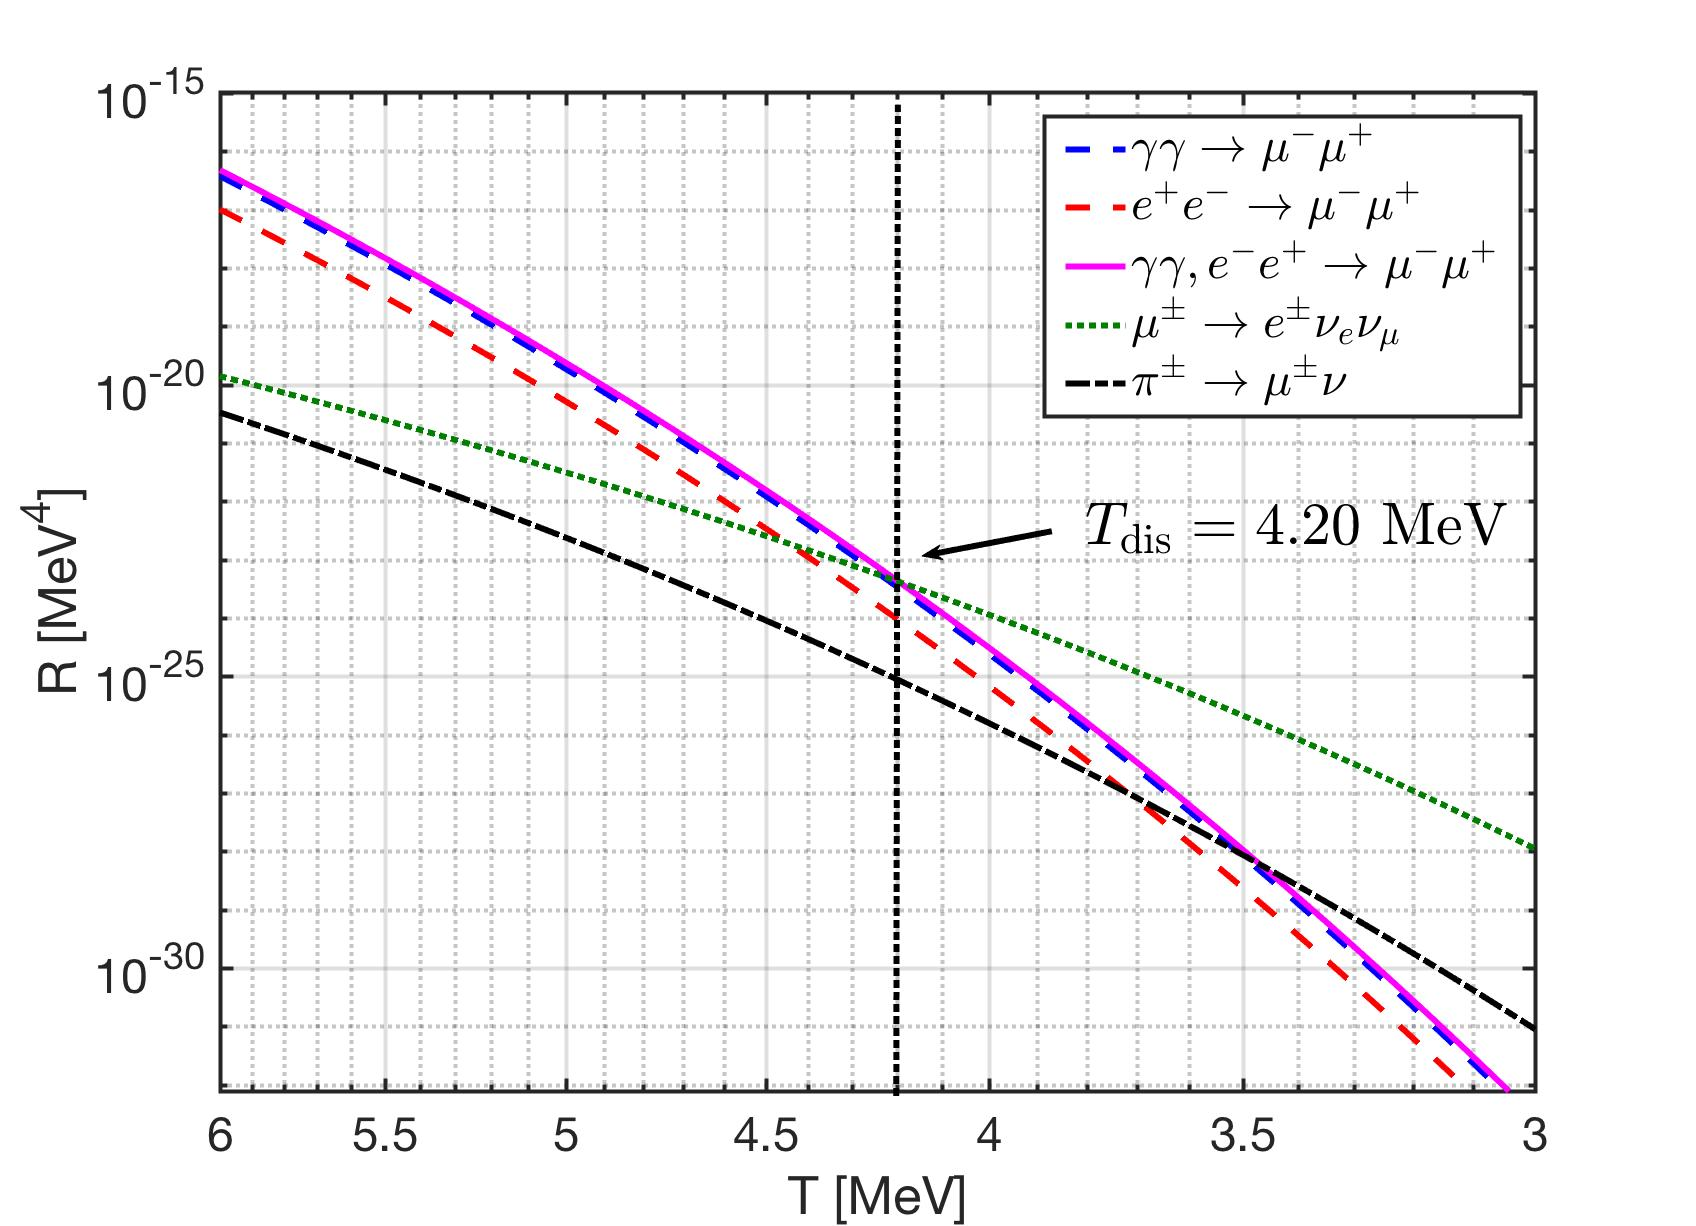
\includegraphics[width=0.9\textwidth]{./plots/MuonRate_new2.jpg}}
\caption{The thermal reaction rate per unit time and units volume for different reactions as a function of temperature. The dominant reactions for $\mu^\pm$ production are ${\gamma+\gamma\to\mu^++\mu^-}$ and $e^++e^-\to\mu^++\mu^-$, and the total production rate crosses the decay rate of $\mu^\pm$ at temperature $T_{dissapear}\approx 4.195$\,MeV. \cccite{Rafelski:2023emw}. \radapt{Yang:2024ret,Rafelski:2021aey}}
\label{MuonRatenew:fig} 
\end{figure}
%%%%%%%%%%%%%%%%%%%%%%%%%%%%%%

Considering the number density for nonrelativistic $\mu^\pm$ in the Boltzmann approximation, we obtain
\begin{align}\label{nmupm}
n_{\mu^\pm}=\frac{g_{\mu^\pm}}{2\pi^2}T^3\left(\frac{m_\mu}{T}\right)^2 K_2(m_\mu/T)=g_{\mu^\pm}\left(\frac{m_\mu T}{2\pi}\right)^{3/2}e^{-{m_\mu}/{T}}\;. 
\end{align}
The ration of the number density between $n_{\mu^\pm}$ and the  baryon $n_B$ can be written as follows
\begin{align}
\frac{n_{\mu^\pm}}{n_\mathrm{B}}=\frac{n_{\mu^\pm}}{s}\frac{s}{n_\mathrm{B}}=
\frac{n_{\mu^\pm}}{s}\left[\frac{s}{n_\mathrm{B}}\right]_{t_0},
\end{align}
where we assume that $s/n_\mathrm{B}$ the ration of entropy to baryon number remains constant and $t_0$ represent present day value. The present value is given by $(n_B/s)_{t_0}\approx8.69\times10^{-11}$\index{baryon!entropy ratio}. We recall, see \rf{EntropyDOF:Fig}, that the entropy density $s$ can be characterized introducing $g^s_\ast$, the total number of \lq entropic\rq\ degrees of freedom
\begin{align}%\label{entrop}
s=\frac{2\pi^2}{45}g^s_\ast T^3\;.
\end{align}
For temperature $10\,\mathrm{MeV} >T>3 $\,MeV, the massless photons, nearly relativistic electron and positrons, and practically massless neutrinos contribute to the degree of freedom $g^s_\ast$.  In this case, the number density between $n_{\mu^\pm}$ and baryon $n_B$ in the temperature interval we consider $10\,\mathrm{MeV} >T>3 $\,MeV is given by
\begin{align}\label{nmuperbF} 
\frac{n_{\mu^\pm}}{n_\mathrm{B}}=\frac{45}{2\pi^2}\frac{g_{\mu^\pm}}{g^s_\ast}\left(\frac{m_\mu}{2\pi T}\right)^{3/2}e^{-{m_\mu}/{T}}\;\left(\frac{s}{n_\mathrm{B}}\right)_{\!t_0}.
\end{align}

%%%%%%%%%%%%%%%%%%%%%%%%%%%%%%%%%
\para{Comparison of muon and baryon abundance}
In \rf{fig:DensityRatio} we show the muon to baryon density ratio \req{nmuperbF} as a function of $T$\index{muon!to baryon ratio}. We see that the very small muon pair abundance at $T=10$\,MeV exceeds that of residual baryons by a factor 500,000 while at muon disappearance temperature $n_{\mu^\pm}/n_\mathrm{B}(T_\mathrm{disappear})\approx0.911$. The number density $n_{\mu^\pm}$ and $n_\mathrm{B}$  abundances are equal at around the temperature $T_\mathrm{equal}\approx4.212\,\mathrm{MeV} >  T_\mathrm{disappear}$.  This means that the muon abundance may still be able to influence baryon evolution because their number density is comparable to the baryon density. Note that we tacitly assumed that the charge asymmetry balancing the charge in protons is contained in the much more abundant electron-positron pairs, this hypothesis needs to be revisited in the future. % However, we also find that at the temperature $T_\mathrm{equal}\approx4.212$\,MeV the density ratio is unity $n_{\mu^\pm}/n_\mathrm{B}\approx1$.

%%%%%%%%%%%%%%%%%%%%%%%%%%%%%%%%%%%%%
\begin{figure}
\centerline{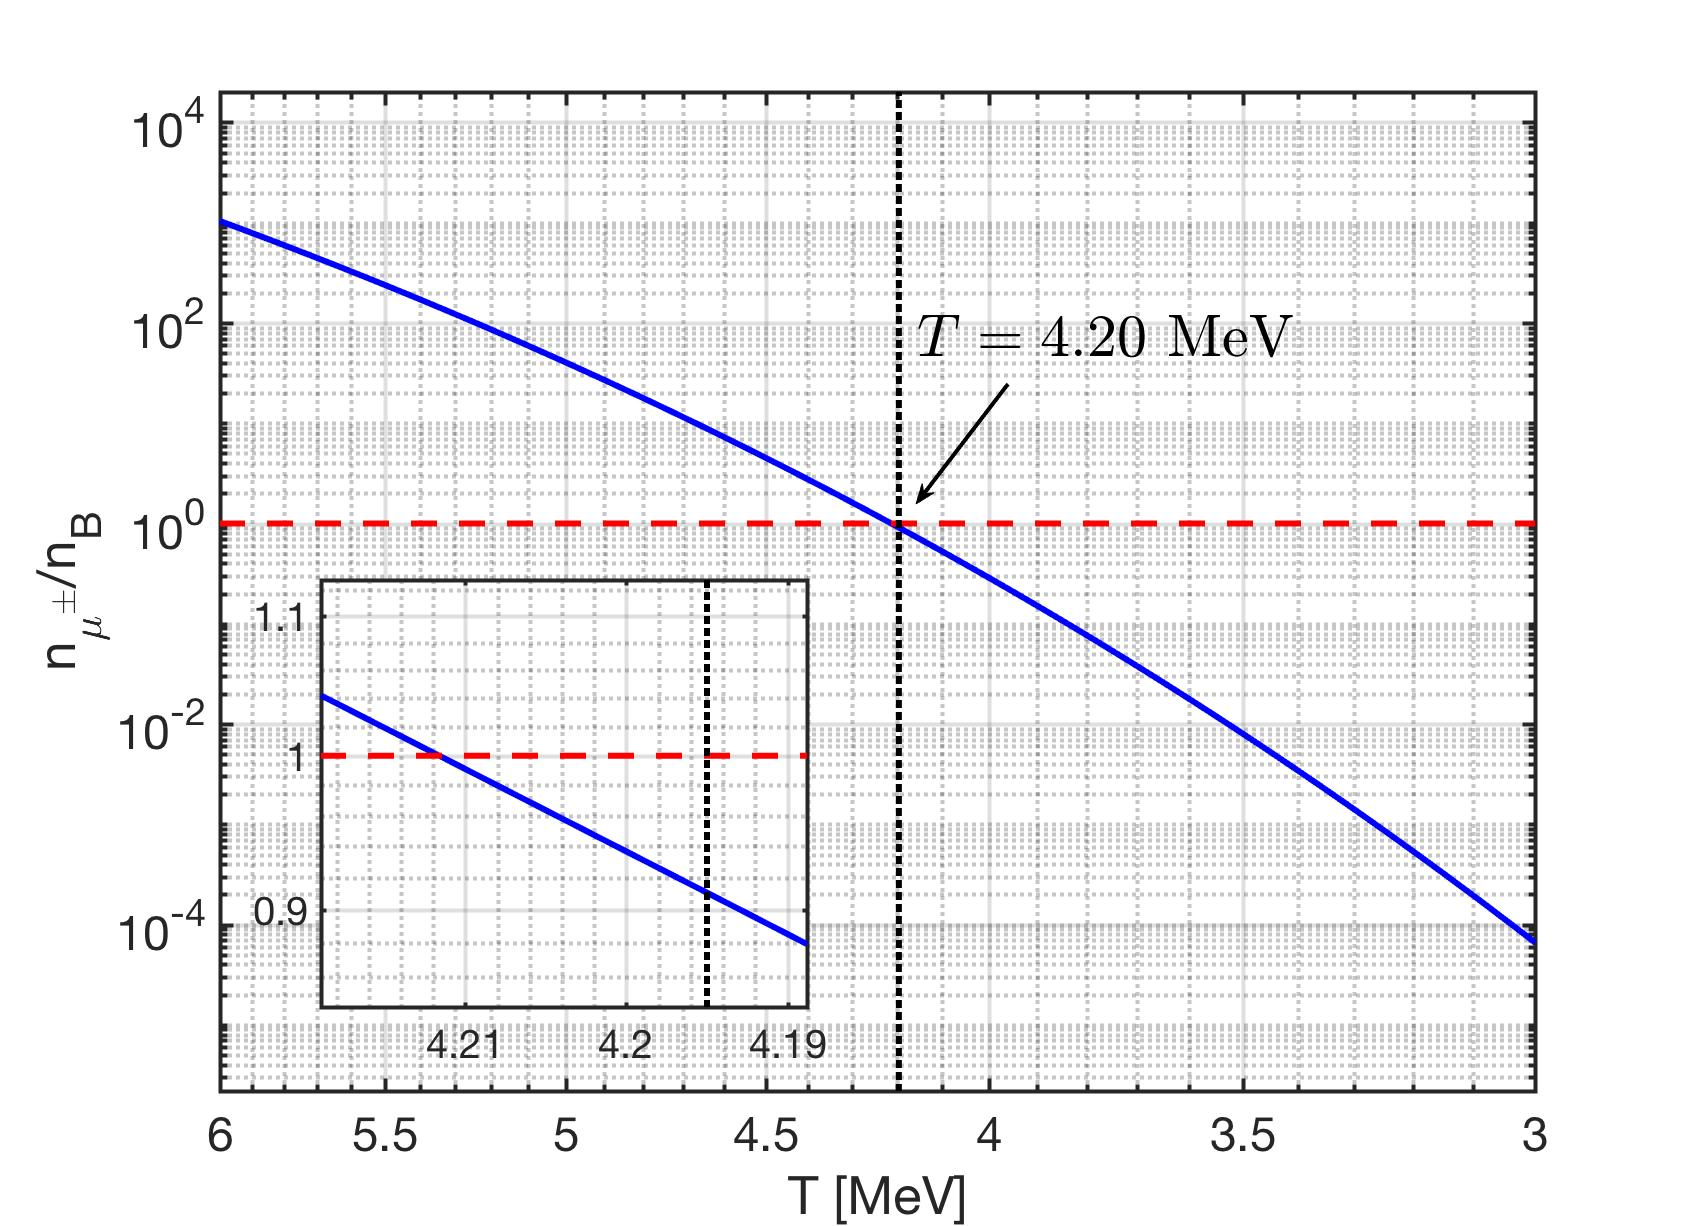
\includegraphics[width=0.9\textwidth]{./plots/DensityRatio_new2.jpg}}
\caption{The density ratio between $\mu^\pm$ and baryons as a function of temperature. The density ratio at muon disappearance temperature is about $n_{\mu^\pm}/n_\mathrm{B}(T_\mathrm{disappear})\approx0.911$, and around the temperature $T\approx4.212$\,MeV the density ratio $n_{\mu^\pm}/n_\mathrm{B}\approx1$. \cccite{Rafelski:2023emw}. \radapt{Yang:2024ret,Rafelski:2021aey}}
\label{fig:DensityRatio}
\end{figure}
%%%%%%%%%%%%%%%%%%%%%%%%

The primary insight of this work is that aside of protons, neutrons and other nonrelativistic particles, both positively and negatively charged muons $\mu^\pm$ are present in thermal equilibrium and in non-negligible abundance exceeding baryon abundance down to  $T>T_\mathrm{dissapear}\approx 4.195$\,MeV. This offers a new and tantalizing model building opportunity for anyone interested in baryon-antibaryon separation in the primordial Universe, strangelet formation, and perhaps other exotic primordial structure formation mechanisms. 



%%%%%%%%%%%%%%%%%%%%%%%%%%%%%%%%%%%%%%%%%%%%%%%
%%%%%%%%%%%%%%%%%%%%%%%%%%%%%%%%%%%%%%%%%%%%%%%
\subsection{Electron-positron plasma and BBN}
\label{section_electron}
Following on the neutrino freeze-out at $T\approx 2$\,MeV, the Universe is dominated by the electron-positron-photon QED plasma. In this section, we derive the electron-positron density and chemical potential required for local charge neutrality\index{charge!neutrality} of the Universe to show that during the normal BBN temperature range $86.7\,\mathrm{keV}>\mathrm{T_{BBN}}>50\,\mathrm{keV}$~\cite{Pitrou:2018cgg} the Universe was filled with a dense electron-positron pair-plasma dotted with a dispersed baryonic matter dust. We then examine the microscope collision properties of the electron-positron plasma in the early Universe allowing us to use  appropriately generalized methods of plasma physics in a study of the role of the $e^+e^-$ plasma in the Universe. The time scale of Universe expansion $H^{-1}$ is orders of magnitude larger than the microscopic reaction time scales of interest for all processes we consider, the dynamical processes we consider are  thus occurring in expanding, but stationary Universe.

%Before BBN, for temperatures $T>86.7\,$keV were high enough that any nuclei formed to be disassociated by the vast number of high energy photons present~\cite{Pitrou:2018cgg}. 
%Once the temperature cooled to around $T<50\,$keV most of the nuclear reactions forming nuclei had already occurred. 
  
%We also note that at this point neutrinos have become free streaming~\cite{Birrell:2012gg}.

%In Ref.\,\cite{Grayson:2022asf} we used the present-day baryon-to-photon ratio: $B/N_\gamma =n_B/n_\gamma= 6.05\times10^{-10}$ from Cosmic Microwave Background (CMB)~\cite{ParticleDataGroup:2022pth} and the charge neutrality of the universe to find the electron-positron chemical potential and density during BBN.
%%%%%%%%%%%%%%%%%%%%%%%%%%%%%%%%%%%%%%%%%
%\begin{figure}  
%\includegraphics[width=0.95\linewidth]{Chemical_Plasma}
%\includegraphics[width=0.95\linewidth]{Density_Plasma002}
%\centerline{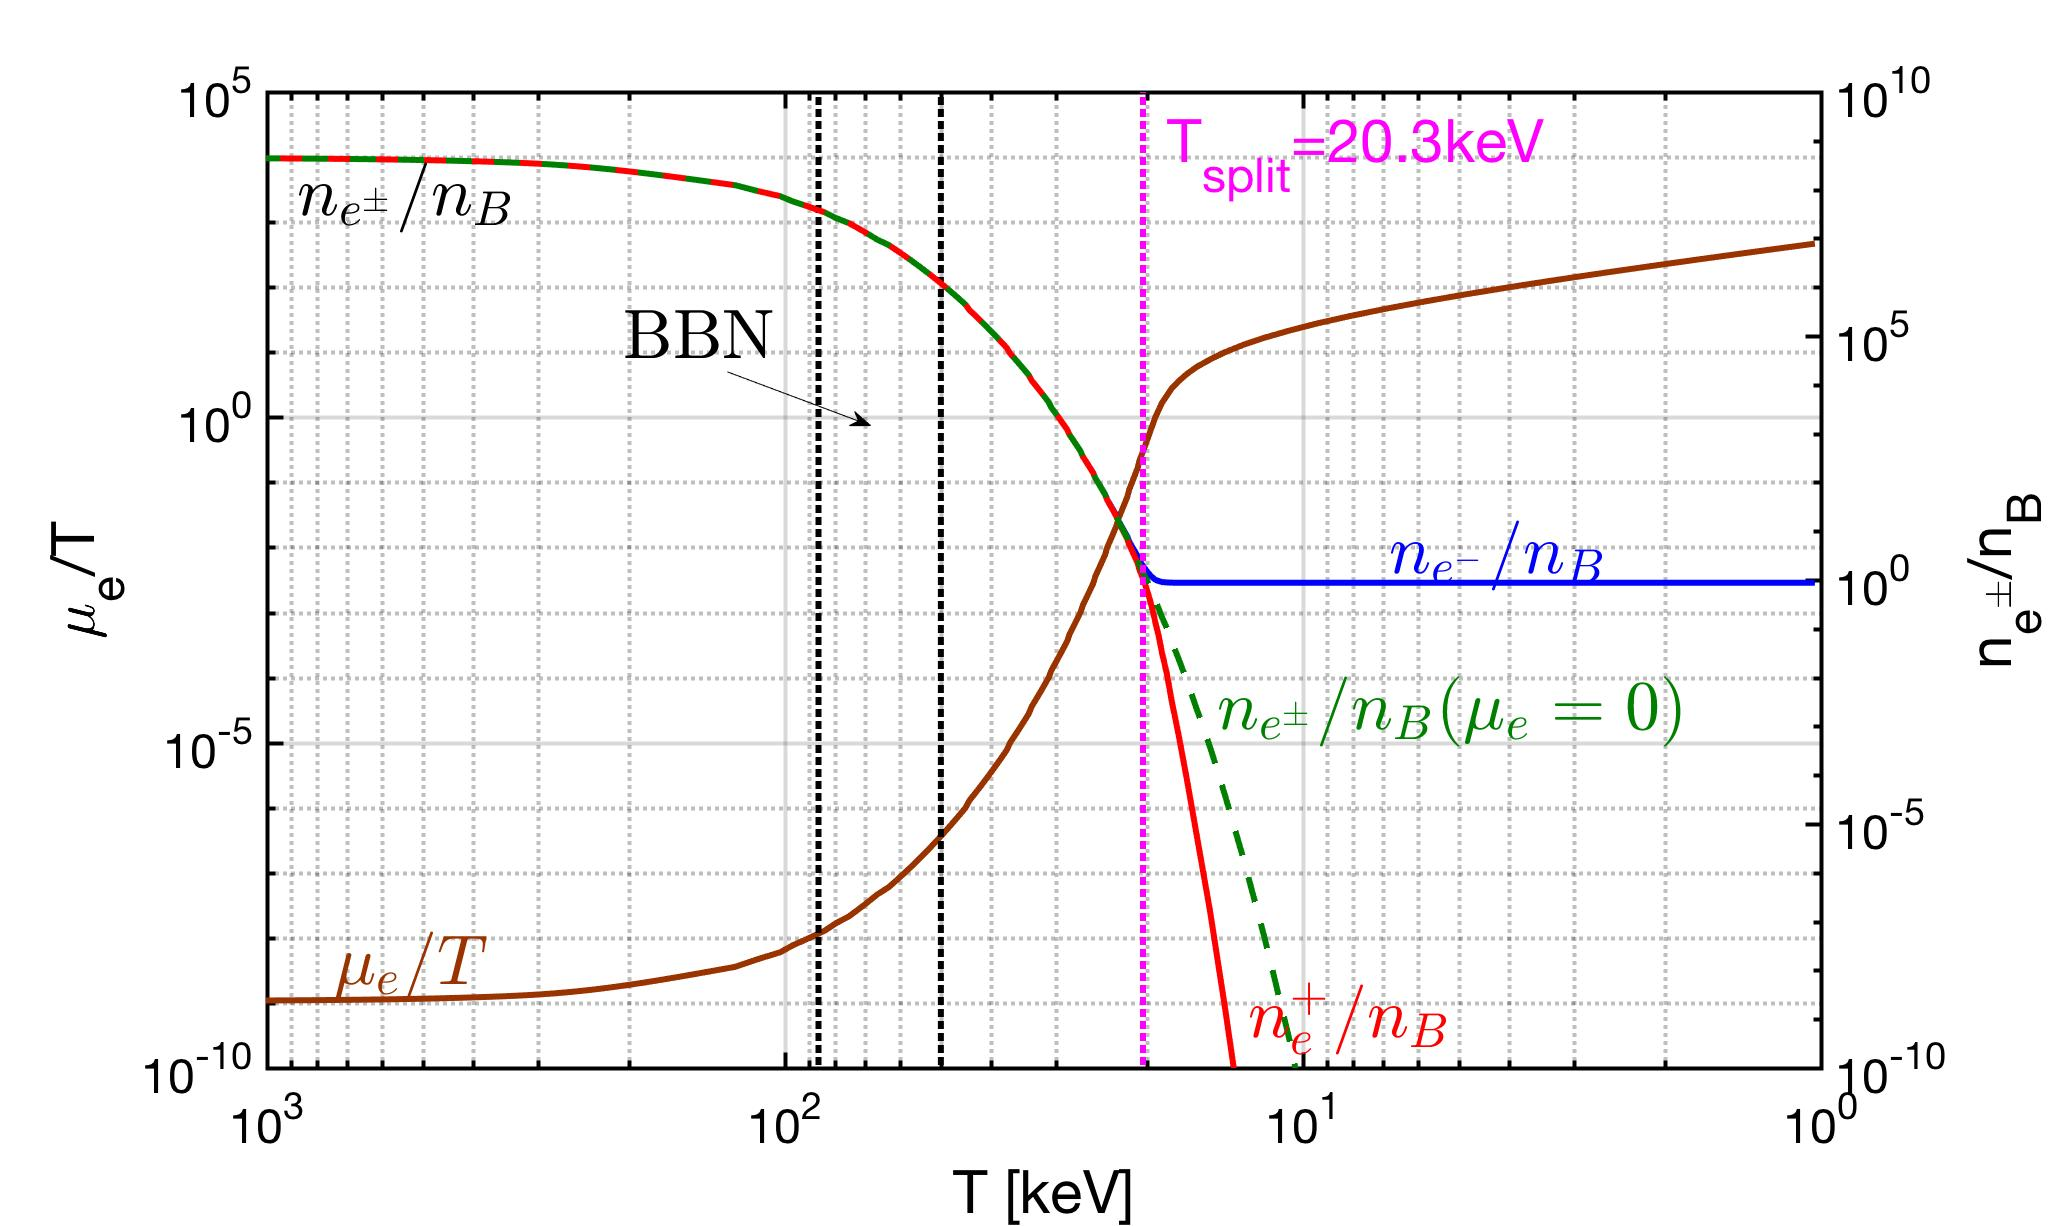
\includegraphics[width=0.90\linewidth]{plots/chap03BBN/May152023_EPDensity_Chemical}}
%\caption{\cccite{Grayson:2023flr}, adapted from Ref.~\cite{Grayson:2023flr} and thesis of C.T.\,Yang~\cite{Yang:2024ret}. Left axis: The chemical potential of electrons as a function of temperature. Right axis: the ratio of electron (positron) number density to baryon density as a function of temperature. The solid blue line is the electron density, the red dashed line is the positron density, and the green dotted line is the number density with $\mu_e=0$. When $T=20.3\,\mathrm{keV}$ (the purple vertical line) positron density decreases rapidly because of the annihilation. The vertical black dotted lines represent BBN temperature range $86\,\mathrm{keV}>\mathrm{T_{BBN}}>50\,\mathrm{keV}$}
%\label{BBN_Electron} 
%\end{figure}
%%%%%%%%%%%%%%%%%%%%%%%%%%%%%%%%%%%%%%%%%%%%%%%%%%%%%

%In \rf{BBN_Electron} (left axis), we plot the electron chemical potential as a function of temperature. We can see the value of chemical potential is comparatively small $\mu_e/T\approx10^{-6}\sim10^{-7}$ during the BBN temperature range, implying an equal number of electrons and positrons in plasma. Thus, for the proceeding calculations, we will set $\mu =0$. When the temperature is around $T=70\,\mathrm{keV}$, the density of electrons and positrons is comparatively large $n_{e^\pm}\approx10^7\,n_B$. This indicates that we can assume the universe is filled mainly with electrons and positrons with light nuclei being a very small component of the plasma. Later when the temperature is around $T=20.3\,\mathrm{keV}$, the positron density decreases, transforming the pair-plasma to an electron-baryon plasma.

%%%%%%%%%%%%%%%%%%%%%%%%%%%%%%%%%%%%%%%%%%%%
\para{Electron chemical potential and number density}\index{chemical potential!electron}
We obtain the dependence of electron chemical potential, and hence $e^+e^-$ density, as a function of the photon background temperature $T$ by employing the following physical principles
\begin{enumerate}
\item Charge neutrality of the Universe:
\begin{align}\label{neutrality}
n_{e^-}-n_{{e^+}}=n_p-n_{\overline{p}}\approx\,n_p,
\end{align}
where $n_\ell$ denotes the number density of particle type $\ell$.
\item Neutrinos decouple (freeze-out) at a temperature $T_f\simeq 2$\,MeV, after which they free stream through the Universe with an effective temperature~\cite{Birrell:2012gg}\index{neutrino!free stream}
\begin{align}
 T_\nu(t)=T_f\,\frac{a(t_f)}{a(t)},
\end{align}
where $a(t)$ is the Friedmann-Lema\^{i}tre-Robertson-Walker (FLRW) Universe scale factor (see cosmology primer \rsec{sec:flrw}) which is a function of cosmic time $t$, and $t_f$ represents the cosmic time when neutrino freezes out.
\item The total comoving entropy\index{comoving!entropy} is conserved. At $T\leq T_f$, the dominant contributors to entropy are photons, $e^+e^-$, and neutrinos. In addition, after neutrino freeze out, neutrino comoving entropy is independently conserved~\cite{Birrell:2012gg}. This implies that the combined comoving entropy in $e^+e^-\gamma$ is also conserved for $T\leq T_f$.\index{entropy!conservation}
\end{enumerate} 
Motivated by the fact that comoving entropy in $\gamma$, $e^+e^-$ is conserved after neutrino freeze-out, we rewrite the charge neutrality condition, \req{neutrality}, in the form
\begin{align}\label{charge_neutral_cond2}
n_{e^-}-n_{{e^+}}=X_p\frac{n_B}{s_{\gamma,e^\pm}} s_{\gamma,e^\pm},\qquad X_p\equiv\frac{n_p}{n_B},
\end{align}
where $n_B$ is the number density of baryons, $s_{\gamma,e^\pm}$ is the combined entropy density in photons, electrons, and positrons. During the Universe expansion, the comoving entropy and baryon number are conserved quantities; hence the ratio $n_B/s_{\gamma,e^\pm}$ is conserved. We have
\begin{align}
\frac{n_B}{s_{\gamma,e^\pm,}}=\left(\frac{n_B}{s_{\gamma,e^\pm}}\right)_{t_0}\!\!\!\!=\left(\frac{n_B}{s_{\gamma}}\right)_{t_0}\!\!\!\!=\left(\frac{n_B}{n_\gamma}\right)_{t_0}\left(\frac{n_\gamma}{s_{\gamma}}\right)_{t_0},
\end{align}
where the subscript $t_0$ denotes the present day value, and the second equality is obtained by observing that the present day $e^+e^-$-entropy density is negligible compared to the photon entropy density. We can evaluate the ratio introducing the present day baryon-to-photon ratio: $B/N_\gamma =n_B/n_\gamma= 0.605\times10^{-9}$ as obtained from the Cosmic Microwave Background (CMB)~\cite{ParticleDataGroup:2022pth}, and the entropy per particle for a massless boson: $(s/n)_{\mathrm{boson}}\approx 3.602$.

The total entropy density of photons, electrons, and positrons can be written as
\begin{align}\label{entropy_per_baryon}
s_{\gamma,e^\pm}=\frac{2\pi^2}{45}g_\gamma\,T^3+\frac{\rho_{e^\pm}+P_{e^\pm}}{T}-\frac{\mu_e}{T}(n_{e^-}-n_{{e^+}}),
 \end{align}
where $ \rho_{e^\pm}=\rho_{e^-}+\rho_{e^+}$ and $P_{e^\pm}=P_{e^-}+P_{{e^+}}$ are the total energy density and pressure of electrons and positron respectively.

By incorporating \req{charge_neutral_cond2} and \req{entropy_per_baryon}, the charge neutrality condition can be expressed as
\begin{align}\label{charge_neutral_cond3}
 &\left[1+X_p\left(\frac{n_B}{n_\gamma}\right)_{t_0}\left(\frac{n_\gamma}{s_{\gamma}}\right)_{t_0}\frac{\mu_e}{T}\right]\frac{n_{e^-}-n_{{e^+}}}{T^3}\notag\\
 &\qquad\qquad\qquad=X_p\left(\frac{n_B}{n_\gamma}\right)_{t_0}\left(\frac{n_\gamma}{s_{\gamma}}\right)_{t_0} \left(\frac{2\pi^2}{45}g_\gamma+\frac{\rho_{e^\pm}+P_{e^\pm}}{T^4}\right).
\end{align}

Using Fermi distribution, the number density of electrons over positrons in the early Universe is given by
\begin{align}\label{ee_density}
n_{e^-}-n_{{e^+}}&=\frac{g_e}{2\pi^2}\left[\int_0^\infty\frac{p^2dp}{\exp{\left((E-\mu_e)\right)/T}+1}\right.\left.-\int_0^\infty\frac{p^2dp}{\exp{\left((E+\mu_e)/T\right)}+1}\right]\notag\\
&=\frac{g_e}{2\pi^2}\,{T^3}\,\tanh(b_e)M_e^3\int_{1}^\infty \!\!\!\!\frac{ \eta \sqrt{\eta^2-1} d\eta}{1+\cosh(M_e\eta)/\cosh(b_e)},
\end{align}
where we have introduced the dimensionless variables as follows: 
\begin{align}\label{Variables}
\eta=\frac{E}{m_e},\qquad M_e=\frac{m_e}{T},\qquad b_e=\frac{\mu_e}{T}.
\end{align}
Substituting \req{ee_density} into \req{charge_neutral_cond3} and giving the value of $X_p$, then the charge neutrality condition can be solved to determine $\mu_e/T$ as a function of $M_e$ and $T$. 

%%%%%%%%%%%%%%%%%%%%%%%%%%%%%%%%%%%%%%%%%%%%%%%%%%%%%%
\begin{figure}
% %\includegraphics[width=0.95\linewidth]{Chemical_Plasma}
% %\includegraphics[width=0.95\linewidth]{Density_Plasma002}
\centerline{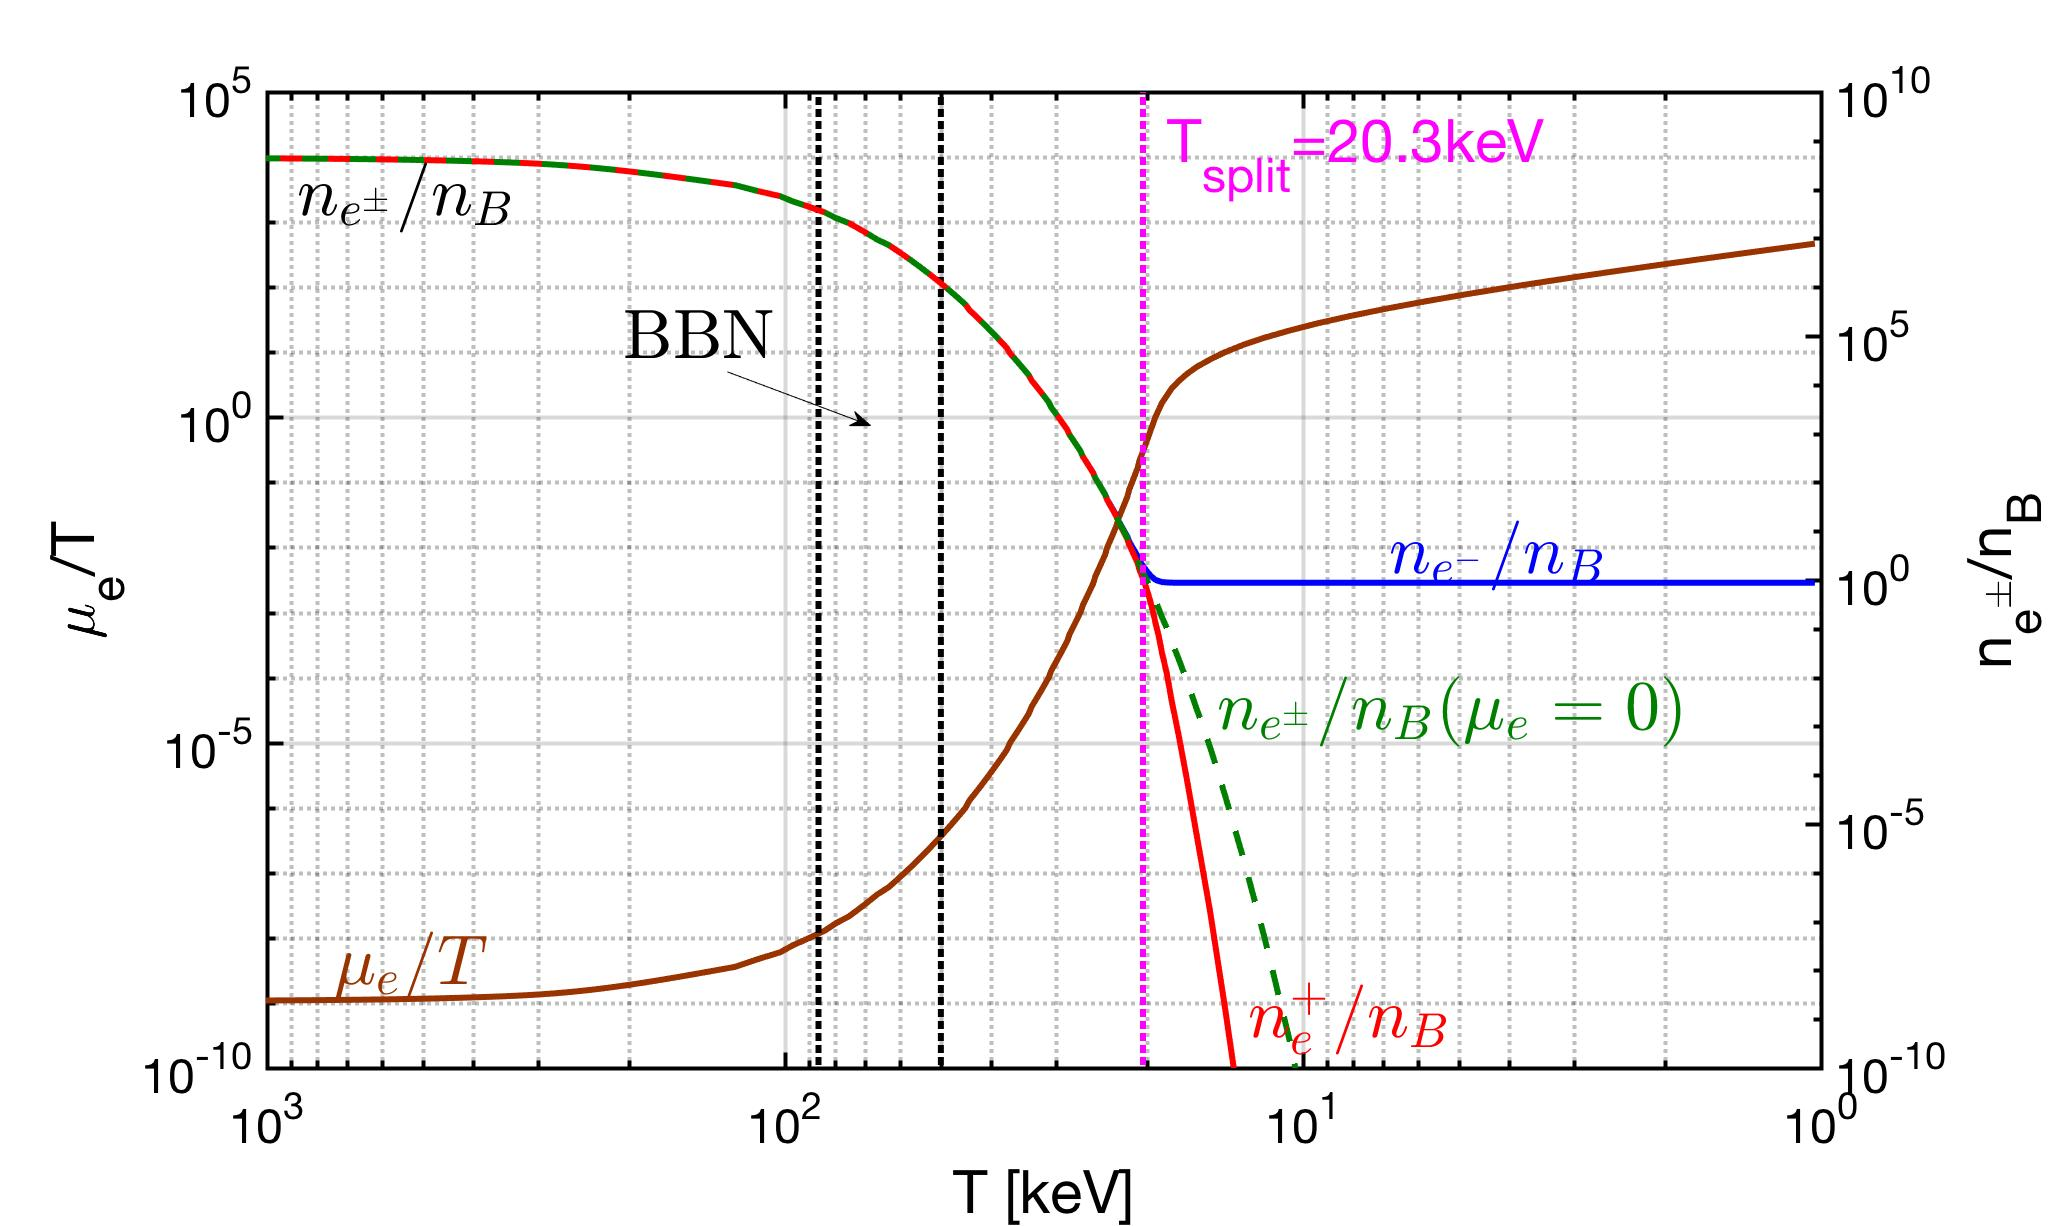
\includegraphics[width=0.90\textwidth]{plots/chap03BBN/May152023_EPDensity_Chemical}}
\caption{Left axis: The chemical potential of electrons as a function of temperature (brown line). Right axis: the ratio of electron (positron) number density to baryon density as a function of temperature. The solid blue line is the electron density, the red  line is the positron density, and the green dashed line is obtained setting for comparison $\mu_e=0$. The vertical black dotted lines are bounds of BBN epoch}
\label{BBN:Electron}
\end{figure}
%%%%%%%%%%%%%%%%%%%%%%%%%%%%%%%%%

In \rf{BBN:Electron} (left axis), we show (left axis, brown line) the electron chemical potential as a function of temperature we obtain solving \req{charge_neutral_cond3} numerically employing the following parameters: proton concentration $X_p=0.878$ as derived from observation~\cite{ParticleDataGroup:2022pth} and $n_B/n_\gamma=6.05\times10^{-10}$ from CMB. We can see the value of chemical potential is comparatively small $\mu_e/T\approx10^{-6}\sim10^{-7}$ during the BBN epoch temperature range, implying a very small asymmetry in the number of electrons and positrons in plasma is needed to neutralize proton charge. 

The ratio of electron (positron) number density to baryon density (right axis) shows that the Universe was filled with an electron-positron rich plasma during the BBN temperature range epoch here set in the temperature range $86\,\mathrm{keV}>\mathrm{T_{BBN}}>50\,\mathrm{keV}$. When the temperature is {\it e.g.\/} around $T=70\,\mathrm{keV}$, the density of electrons and positrons is comparatively large $n_{e^\pm}\approx10^7\,n_B$. At $90$\,keV, the electron and positron density is near the solar core density, compare Fig.~19 in Ref.~\cite{Rafelski:2023emw}. Near and below   the temperature  $T=20.3\,\mathrm{keV}$, the positron density decreases rapidly, transforming the pair-plasma into an electron-baryon plasma.

%%%%%%%%%%%%%%%%%%%%%%%%%%%%%%%%%%%%%%%%%%%%
\para{QED plasma damping rate}
\index{plasma!QED damping}
The reactions of interest for the evaluation of the QED plasma damping are the (inverse) Compton scattering, the M{\o}ller scattering, and the Bhabha scattering, respectively
\begin{align}
e^\pm+\gamma\longrightarrow e^\pm+\gamma,\qquad e^\pm+e^\pm\longrightarrow e^\pm+e^\pm,\qquad e^\pm+e^\mp\longrightarrow e^\pm+e^\mp.
\end{align}
The general formula for thermal reaction rate per volume is discussed in~\cite{Letessier:2002ony} (Eq.(17.16), Chapter 17). For inverse Compton scattering we have
\begin{align}
R_{e^{\pm}\gamma}=\frac{g_eg_\gamma}{16\left(2\pi\right)^5}T\int_{m_e^2}^\infty\!\!\!\!ds\frac{K_1(\sqrt{s}/T)}{\sqrt{s}}\int^0_{-(s-m_e^2)^2/s}\!\!\!\!\!\!dt\, |M_{e^{\pm}\gamma}|^2,
\end{align} 
and for M{\o}ller and Bhabha reactions we have
\begin{align}
&R_{e^\pm e^\pm}=\frac{g_eg_e}{16\left(2\pi\right)^5}T\!\!\int_{4m_e^2}^\infty\!\!\!\!ds\frac{K_1(\sqrt{s}/T)}{\sqrt{s}}\int^0_{-(s-4m_e^2)}\!\!\!\!\!\!dt\,|M_{e^\pm e^\pm}|^2,\\[0.3cm]
&R_{e^\pm e^\mp}=\frac{g_eg_e}{16\left(2\pi\right)^5}T\!\!\int_{4m_e^2}^\infty\!\!\!\!ds\frac{K_1(\sqrt{s}/T)}{\sqrt{s}}\int^0_{-(s-4m_e^2)}\!\!\!\!\!\!dt\,|M_{e^\pm e^\mp}|^2,
\end{align}
where $g_i$ is the degeneracy of particle $i$, $|M|^2$ is the matrix element for a given reaction, $K_1$ is the Bessel function of order $1$, and $s,t,u$ are Mandelstam variables\index{Mandelstam!variables}. The leading order matrix element associated with inverse Compton scattering can be expressed in the Mandelstam variables~\cite{Kuznetsova:2011wt,Kuznetsova:2009bq} we have\index{Compton!inverse scattering}
\begin{align}
|M_{e^\pm\gamma}|^2\!=32 \pi^2\alpha^2\bigg[&4\left(\frac{m_e^2}{m_e^2-s}+\frac{m_e^2}{m_e^2-u}\right)^2\notag\\
&\qquad\qquad-\frac{4m_e^2}{m_e^2-s}-\frac{4m_e^2}{m_e^2-u} -
 \frac{m_e^2-u}{m_e^2-s} -\frac{m_e^2-s}{m_e^2-u}\bigg],
\end{align}
and for M{\o}ller\index{M{\o}ller!scattering} and Bhabha scattering we have \index{Bhabha!scattering}
\begin{align}
|M_{e^{\pm}e^{\pm}}|^{2}\!=64\pi^{2}\alpha^{2}\bigg[&
\frac{s^{2}+u^{2}+8m_e^{2}(t-m_e^{2})}{2(t-m^2_{\gamma})^{2}}\notag\\
&\quad+\frac{{s^{2}+t^{2}}+8m_e^{2}
(u-m_e^{2})}{2(u-m_{\gamma}^2)^{2}} + \frac{\left( {s}-2m_e^{2}\right)\left({s}-6m_e^{2}\right)}
{(t-m_{\gamma}^2)(u-m_{\gamma}^2)} \bigg],
\end{align}
and
\begin{align}
|M_{e^\pm e^\mp}|^{2}=64\pi^{2}\alpha^{2}
\bigg[&\frac{s^{2}+u^{2}+8m_e^{2}(t-m_e^{2})}{2(t-m^2_{\gamma})^{2}}\notag\\
&\quad+\frac{u^{2}+t^{2}+8m_e^{2}
(s-m_e^{2})}{2(s-m^2_{\gamma})^{2}}  +   \frac{\left({u}-2m_e^{2}\right)\left({u}-6m_e^{2}\right)}
   {(t-m^2_{\gamma})(s-m^2_{\gamma})} \bigg],
\label{M_fi_b}
\end{align}
where we introduce the photon mass $m_\gamma$ to account the plasma effect and avoid singularity in reaction matrix elements. 

The photon mass $m_\gamma$ in plasma is equal to the plasma frequency $\omega_p$, where we have~\cite{Kislinger:1975uy}\index{photon!plasma mass}
\begin{align}
m^2_\gamma=\omega^2_{p}=8\pi\alpha\int\frac{d^3p_e}{(2\pi)^3}\left(1-\frac{p_e^2}{3E_e^2}\right)\frac{f_e+f_{\bar e}}{E_e},
\end{align}
where $E_e=\sqrt{p_e^2+m^2_e}$. In the BBN temperature range $86\,\mathrm{keV}>T_{BBN}>50\,\mathrm{keV}$ we have $m_e\gg T$ and considering the nonrelativistic limit for electron-positron plasma, we obtain
\begin{align}
m^2_\gamma=\frac{4\pi\alpha}{2m_e}\left(\frac{2m_eT}{\pi}\right)^{3/2}e^{-m_e/T}\cosh\left(\frac{\mu_e}{T}\right).
\end{align}
In the BBN temperature range, we have $\mu_e/T\ll1$, which implies the equal number of electrons and positrons in plasma.

To discuss the collisions plasma by the linear response theory, it is convenient to define the average relaxation rate for the electron-positron plasma as follows:\index{electron-positron plasma!damping rate}
\begin{align}\label{Kappa}
\kappa=\frac{R_{e^\pm e^\pm}+R_{e^\pm e^\mp}+R_{e^\pm\gamma}}{\sqrt{n_{e^-}n_{e^+}}}\approx\frac{R_{e^\pm e^\pm}+R_{e^\pm e^\mp}}{\sqrt{n_{e^-}n_{e^+}}},
\end{align}
where the density function ${\sqrt{n_{e^-}n_{e^+}}}$ in the Boltzmann limit is given by
\begin{align}
{\sqrt{n_{e^-}n_{e^+}}}=\frac{g_e}{2\pi^3}T^3\left(\frac{m_e}{T}\right)^2K_2(m_e/T).
\end{align}

In \rf{RelaxationRate:fig}, we show the reaction rates for M{\o}ller reaction, Bhabha reaction, and inverse Compton scattering as a function of temperature. For temperatures $T>12.0$\,keV, the dominant reactions in plasma are M{\o}ller and Bhabha scatterings between electrons and positrons. Thus in the BBN temperature range, we can neglect the inverse Compton scattering. The total relaxation rate $\kappa$ (black line) is approximately constant, $\kappa=10\sim12$\,keV, during the BBN. However, at $T<20.3$\,keV the relaxation rate $\kappa$ decreases rapidly because the plasma changes its nature when positrons disppear.

%%%%%%%%%%%%%%%%%%%%%%%%%%%%%%%
\begin{figure} 
%\includegraphics[width=0.95\linewidth]{KappaRateToT_May082023}
\centerline{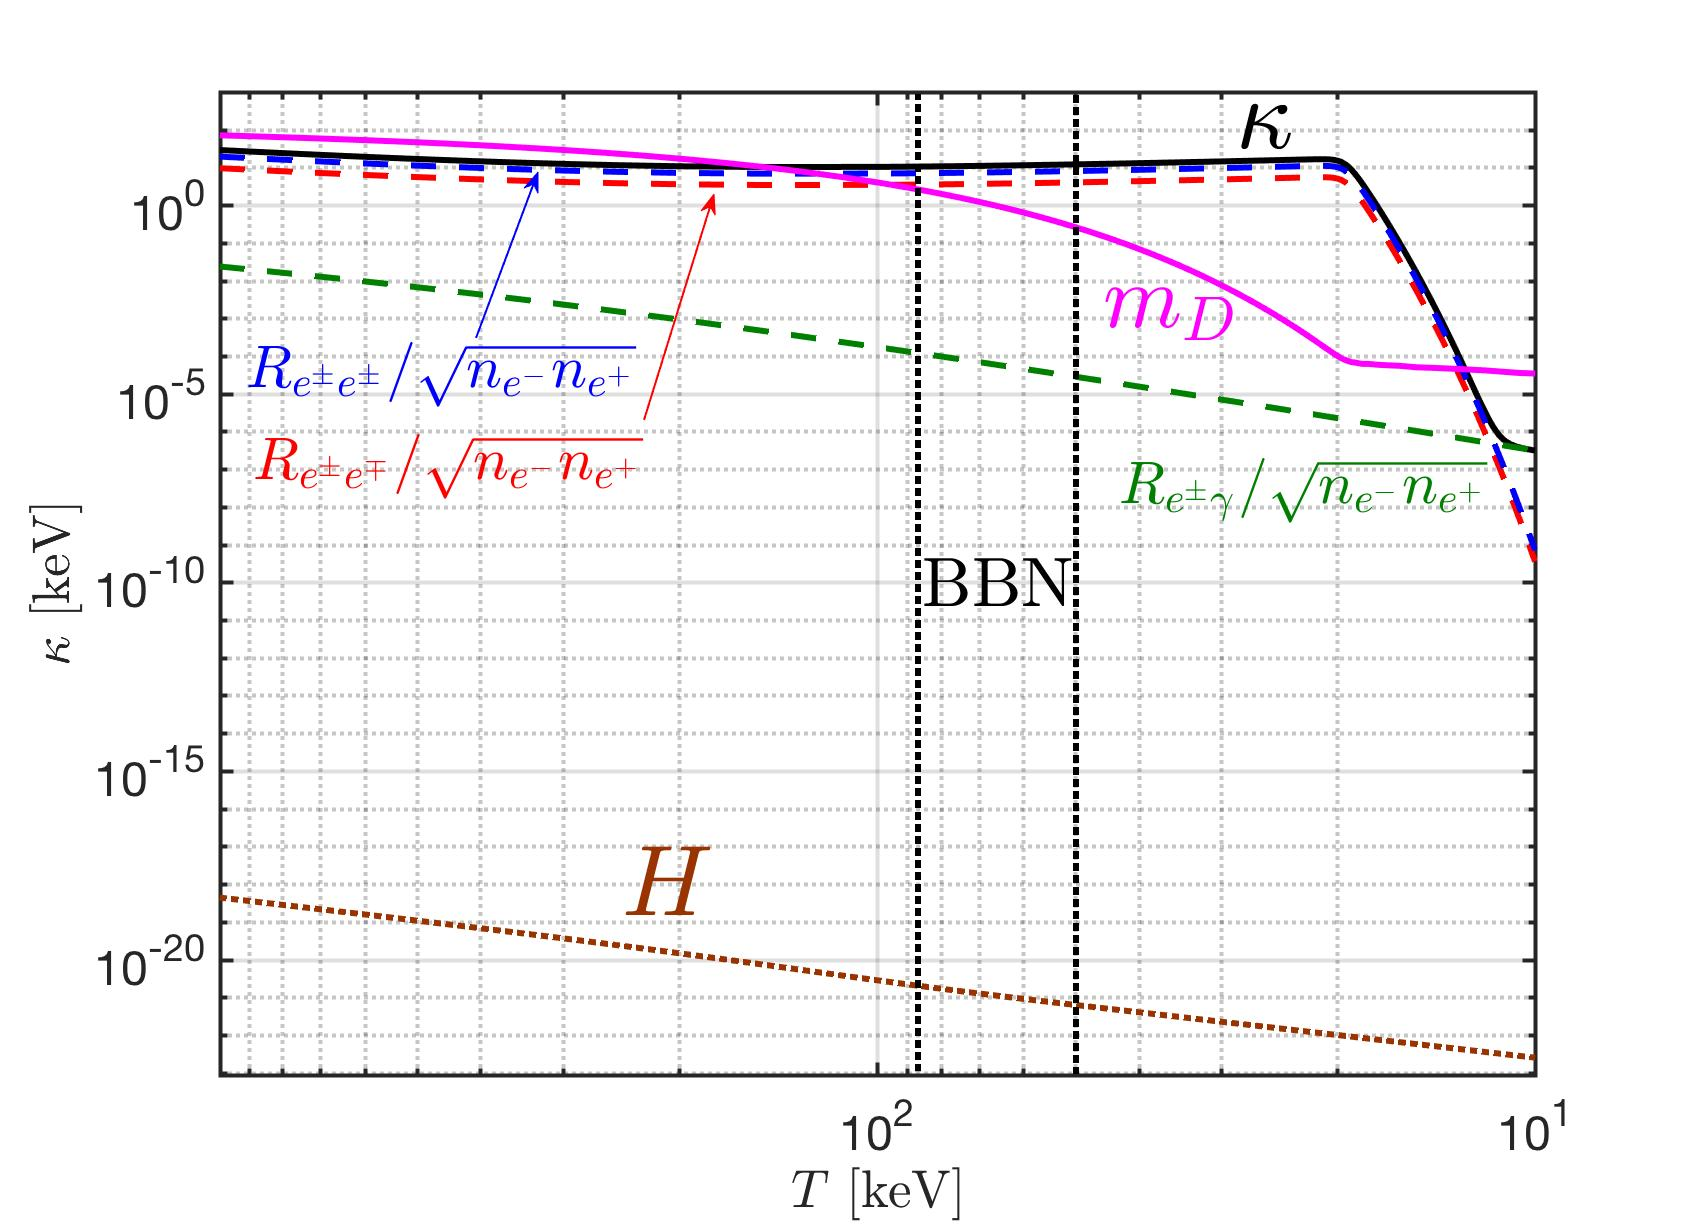
\includegraphics[width=0.9\textwidth]{./plots/May152023Kappa_EPPlasma}}
\caption{The relaxation rate $\kappa$ (black line) as a function of temperature in the nonrelativistic electron-positron plasma, compared to reaction rates  for M{\o}ller reaction $e^-+e^-\to e^-+e^-$ (blue dashed line), Bhabha reaction $e^-+e^+\to e^-+e^+$ (red dashed line), and inverse Compton scattering $e^-+\gamma\to e^-+\gamma$ (green dashed line) respectively. The Debye mass $m_D=\omega_{p}\sqrt{m_e/T}$ (purple line) is also shown. \cccite{Grayson:2023flr}. \radapt{Yang:2024ret}}
\label{RelaxationRate:fig}
\end{figure}
%%%%%%%%%%%%%%%%%%%%%%%%


%%%%%%%%%%%%%%%%%%%%%%%%%%%%%%%
\para{Self-consistent damping rate}
In electron-positron plasma, the photon mass appears as $m_\gamma^2$ in the transition matrices for M{\o}ller and Bhabha reactions, which is one of important parameters in the calculation of the relaxation rate in $e^\pm$ plasma. When evaluating M{\o}ller and Bhabha scattering, we included as is common practice the temperature-dependent mass of the photon obtained in plasma theory without damping. Hwever, in general, the effective mass of the photon depends at a given temperature on all properties of the QED plasma. 

Considering the linear response theory, the dispersion relation for the photon in nonrelativistic $e^\pm$ plasma is given by~\cite{Formanek:2021blc}
\begin{align}\label{dispersion_damping}
w^2=|k|^2+\frac{w}{w+i\kappa}w_{pl}^2,
\end{align}
where $w_{pl}$ is the plasma frequency and $\kappa$ is the average collision rate of $e^\pm$ plasma. The effective plasma frequency in damped plasma can be solved by considering the case $|k|^2=0$~\cite{Formanek:2021blc}
\begin{align}\label{plasmafrequency_damped}
w_{\pm}=-i\frac{\kappa}{2}\pm\sqrt{w^2_{pl}-\frac{\kappa^2}{4}}.
\end{align}
The result shows that the plasma frequency in damped plasma $w_\pm$ is a function of $\kappa$ which we are computing.  

However, the effective photon mass in damped plasma is also a function of the scattering rate. We have
\begin{align}\label{PhotonMass_self}
m_\gamma=w_\pm(w_{pl},\kappa)=m_\gamma(w_{pl},\kappa),
\end{align}
where the photon mass $m_\gamma=w_+$ for the under-damped plasma $w_{pl}>\kappa/2$, and $m_\gamma=w_-$ for over-damped plasma $w_{pl}<\kappa/2$. \req{PhotonMass_self} shows that computed damping strength $\kappa$ is the dominant scale for collisional plasma and it is also the main parameter determining the photon mass in plasma. 

Substituting the effective photon mass  \req{PhotonMass_self} into the definition of the average relaxation rate \req{Kappa}, we obtain a self-consistent equation for damping rate $\kappa$   
\begin{align}\label{RealaxtionSelf}
\kappa\,\left[\frac{g_e}{2\pi^3}T^3\left(\frac{m_e}{T}\right)^2K_2(m_e/T)\right]=\frac{g_eg_e}{32\pi^4}T\!\! \int_{4m_e^2}^\infty\!\!\!\!ds&
\frac{s(s-4m^2_e)}{\sqrt{s}}K_1(\sqrt{s}/T)\times\\&\notag
\bigg[\sigma_{e^\pm e^\pm}(s,w_{pl},\kappa)+\sigma_{e^\pm e^\mp}(s,w_{pl},\kappa)\bigg],
\end{align}
where the cross sections depend on the parameter $w_{pl}$ and $\kappa$, and the variable $\kappa$ appears on both sides of the equation so we need solve the equation numerically to determine the $\kappa$ value that satisfies this condition.


Depending on the nature of the plasma (overdamped or underdamped plasma), we can establish the photon mass in collision plasma based on two distinct conditions as follows:
\begin{itemize}
\item Case 1. The plasma frequency is larger than the collision rate $w_{pl}>\kappa/2$, we have
\begin{align}
m_\gamma=w_+=-i\frac{\kappa}{2}+\sqrt{w^2_{pl}-\frac{\kappa^2}{4}}.
\end{align}
\item Case 2. The plasma frequency is smaller than the collision rate $w_{pl}<\kappa/2$, we have
\begin{align}\label{PhotonMassPlasma}
m_\gamma=w_-=-i\left(\frac{\kappa}{2}+\sqrt{\frac{\kappa^2}{4}-w^2_{pl}}\right).
\end{align}
\end{itemize}
In \rf{RelaxationRate002:fig} we see that during the BBN epoch $50\leqslant T\leqslant 86$\,keV, the plasma frequency is smaller than the collision rate $w_{pl}<\kappa/2$.  In this case, the effective photon mass in collision plasma is given by the overdamped relation \req{PhotonMassPlasma}. For temperature $T<20.3$\,keV, the composition  turns into electron and proton  plasma, which is beyond our current study because of assumed (for simplicity) equal numbers of electrons and positrons.

%%%%%%%%%%%%%%%%%%%%%%%%%%%%%%%%%
\begin{figure}  
%\includegraphics[width=0.95\linewidth]{KappaRateToT_May082023}
\centerline{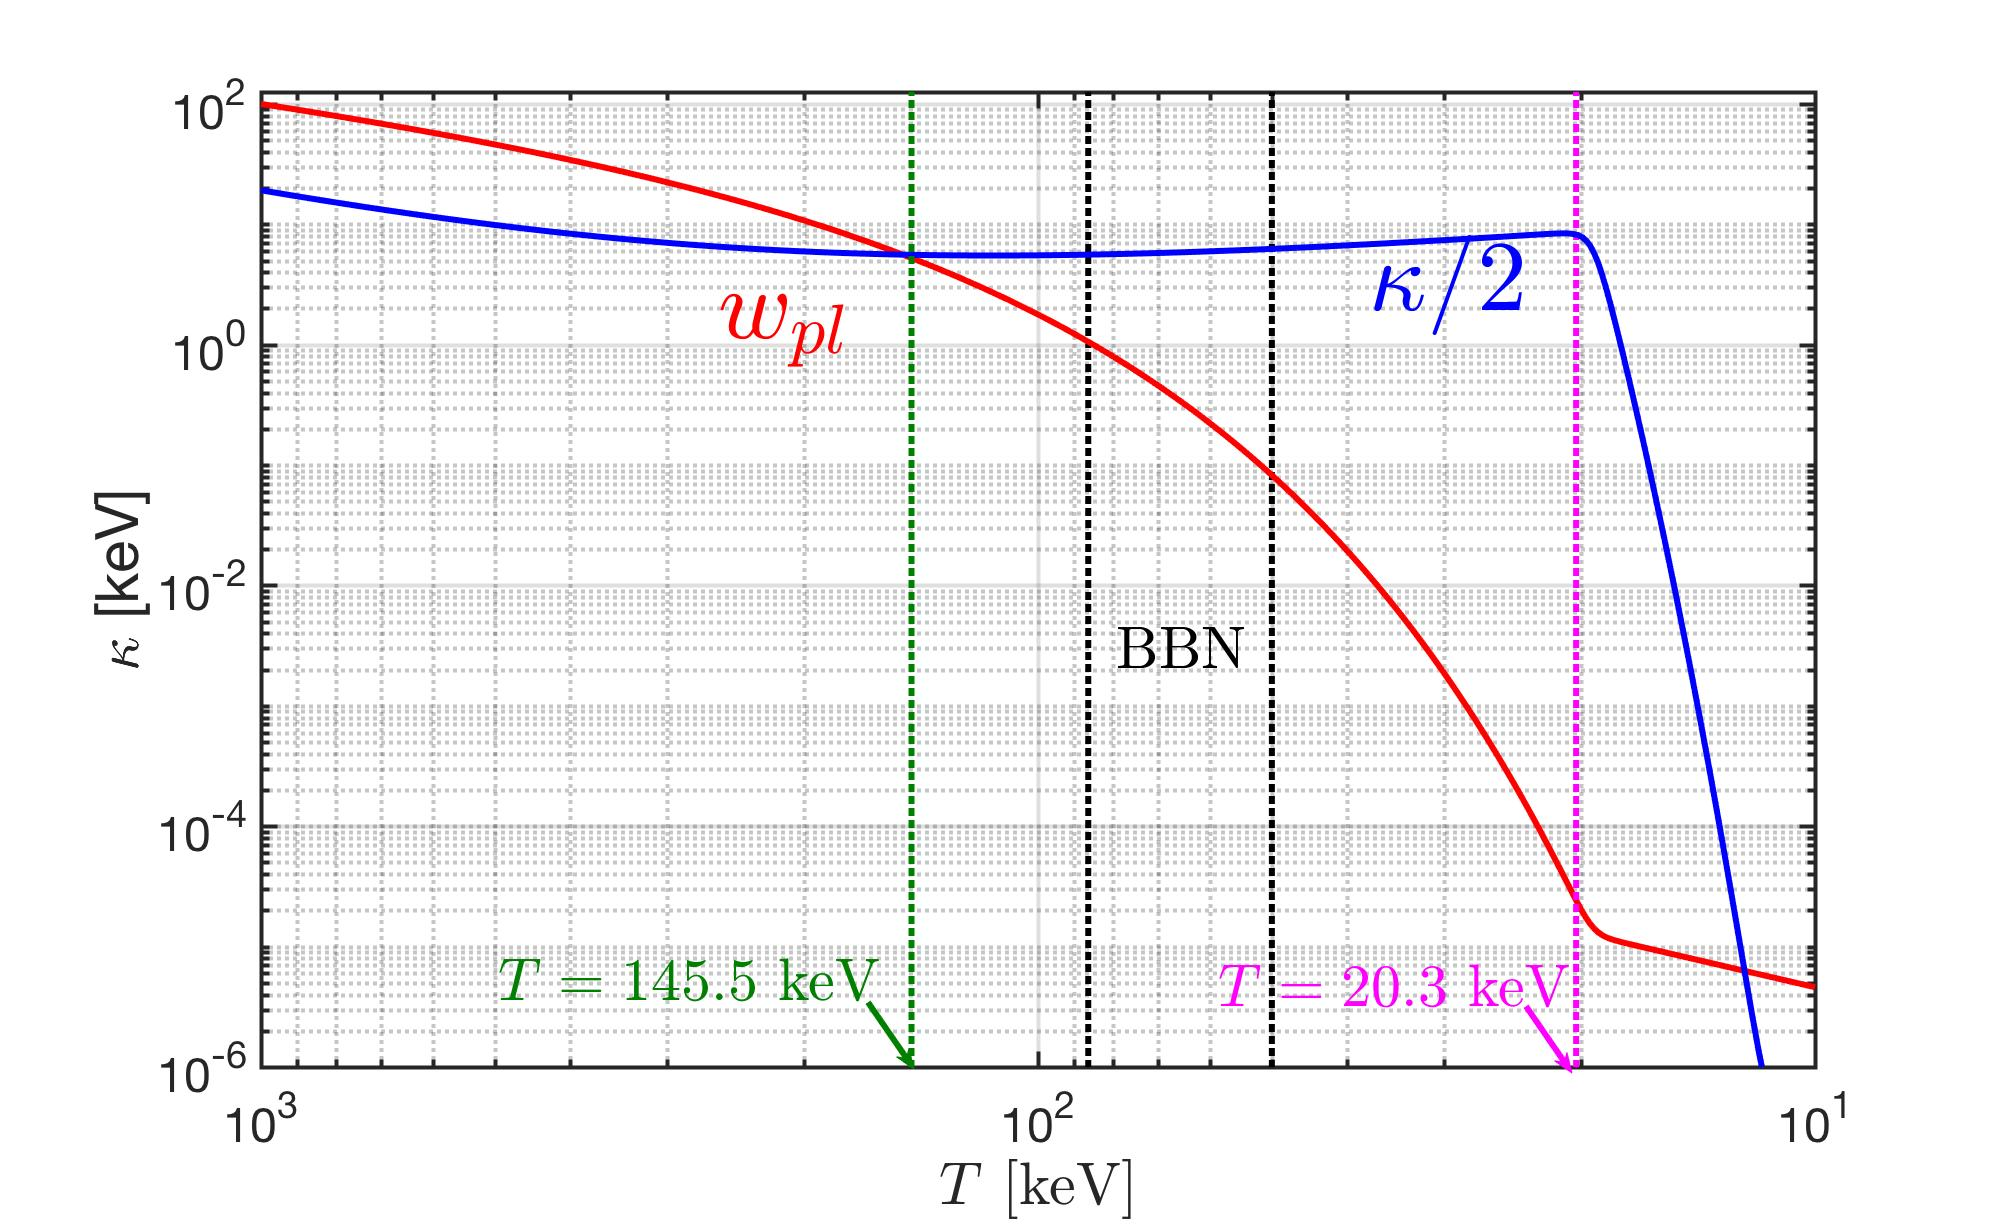
\includegraphics[width=0.9\textwidth]{./plots/KappaElectronPhotonMass_Talk}}
\caption{The relaxation rate $\kappa/2$ (blue line) and plasma frequency $\omega_{pl}$ (red line) as a function of temperature in nonrelativistic electron-positron plasma. Vertical green dashed line indicates the boundary between over- and under-damped plasma at  $T<145.5$\,keV  which is before the BBN epoch (vertical black lines). Temperature domain of validity is above disappearance of positrons (vertical line at 20.3\,keV)}
\label{RelaxationRate002:fig} 
\end{figure}
%%%%%%%%%%%%%%%%%%%%%%%%%%%%%%%%%%%%%%%%%

To calculate the effective cross sections for  M{\o}ller and Bhabha scattering we need in the overdamped regime to account for the imaginary photon mass in the calculation of reaction matrix elements. This imaginary part of the photon mass accounts for the decay in sense  of propagation range of the massive photon in plasma. We now make a first estimate of the effect of self-consistent real part of the photon mass on the damping rate $\kappa$, we leave the photon decay to a future study.

For BBN temperature $50\leqslant T\leqslant 86$\,keV,
we have $w_{pl}<\kappa$ and the effective photon mass can be approximated as
\begin{align}
m^2_\gamma=w_-w_-^\ast&=\left(\frac{\kappa}{2}+\sqrt{\frac{\kappa^2}{4}-w^2_{pl}}\right)^2
=\frac{\kappa^2}{2}\left[\left(1-\frac{2w^2_{pl}}{\kappa^2}\right)+\sqrt{1-\frac{4w^2_{pl}}{\kappa^2}}\right]\notag\\
&=\frac{\kappa^2}{2}\left[\left(1-\frac{2w^2_{pl}}{\kappa^2}\right)+\left(1-\frac{2w^2_{pl}}{\kappa^2}+\cdots\right)\right]\approx\kappa^2.
\label{PhotonMassPlasma002}
\end{align}
where we consider the limit $w^2_{pl}/\kappa^2\ll 1$ and effective photon mass is equal to the average collision rate in plasma $m^2_\gamma\approx\kappa$.

Substituting the photon mass $m^2_\gamma=\kappa^2$ for overdamped plasma into the relaxation rate of electron-positron \req{RealaxtionSelf}, and introducing the following dimensionless variables
\begin{align}
x=\sqrt{s}/T,\qquad a=m_\gamma/T=\kappa/T,\qquad b=m_e/T,
\end{align}
the relaxation rate of electron-positron can be written as
\begin{align}\label{Numerical_eq}
&\left[\frac{g_e}{2\pi^2}T^4\left(\frac{m_e}{T}\right)^{\!2}\!K_2(m_e/T)\right]\,\left(\frac{\kappa}{T}\right)\notag\\
&\qquad\qquad\qquad=\frac{g^2_e\alpha^2}{8\pi^3}T^4\!\!\int_{2b}^\infty\!dxK_1(x)\left[\mathcal{F}_{e^\pm e^\pm}(x,\kappa/T)+\mathcal{F}_{e^\pm e^\mp}(x,\kappa/T)\right],
\end{align}
where the functions $\mathcal{F}_{e^\pm e^\pm}$ and $\mathcal{F}_{e^\pm e^\mp}$ are given by
\begin{align}
\mathcal{F}_{e^\pm e^\pm}(x,a=\kappa/T)&=\left\{2\left[3a^2+4b^2+\frac{4(b^4-a^4)}{x^2-4b^2+2a^2}\right]\ln\left(\frac{a^2}{x^2-4b^2+a^2}\right)\right.\notag\\
&\left.+\frac{(x^2-4b^2)(8b^4+2a^4+3a^2x^2+2x^4-4b^2(2x^2+a^2))}{a^2(x^2-4b^2+a^2)}\right\}
\end{align}
and 
\begin{align}
\mathcal{F}_{e^\pm e^\mp}(x,a=\kappa/T)&=\left\{\frac{2x^2(a^2+x^2)-4b^4}{x^2-a^2}\ln\left(\frac{a^2}{x^2-4b^2+a^2}\right)\right.\notag\\
&+\frac{(x^2-4b^2)(3x^2+4b^2+2a^2)}{(x^2-a^2)}+\frac{x^6-12b^4x^2-16b^6}{3(x^2-a^2)^2}\notag\\
&\left.+\frac{(x^2-4b^2)(8b^4+2a^4+3a^2x^2+2x^4-4b^2(2x^2+a^2))}{a^2(x^2-4b^2+a^2)}\!\right\}.
\end{align}

We solve \req{Numerical_eq} numerically. In \rf{KappaSol:fig}, we plot the resultant relaxation rate $\kappa$ that satisfies \req{Numerical_eq} as a function of temperature $50\,\mathrm{keV} \leqslant T\leqslant 86$\,keV. The result shows that in the the BBN temperature range, the overdamping is considerably reduced: We remember that we started with   $w_{pl}<\kappa$, and the effective photon mass $m^2_\gamma=\kappa^2$. Now we obtain a relaxation rate $\kappa=1.832\sim 0.350$\,keV during  BBN epoch, which is smaller than the relaxation rate without damping effect on the photon mass, compare \rf{RelaxationRate:fig}, where the relaxation rate $\kappa=10\sim12$\,keV during the BBN epoch is shown.

%%%%%%%%%%%%%%%%%%%%%%%%%%%%%%%%%%%%%%%%%%%%%%
\begin{figure} 
\centerline{
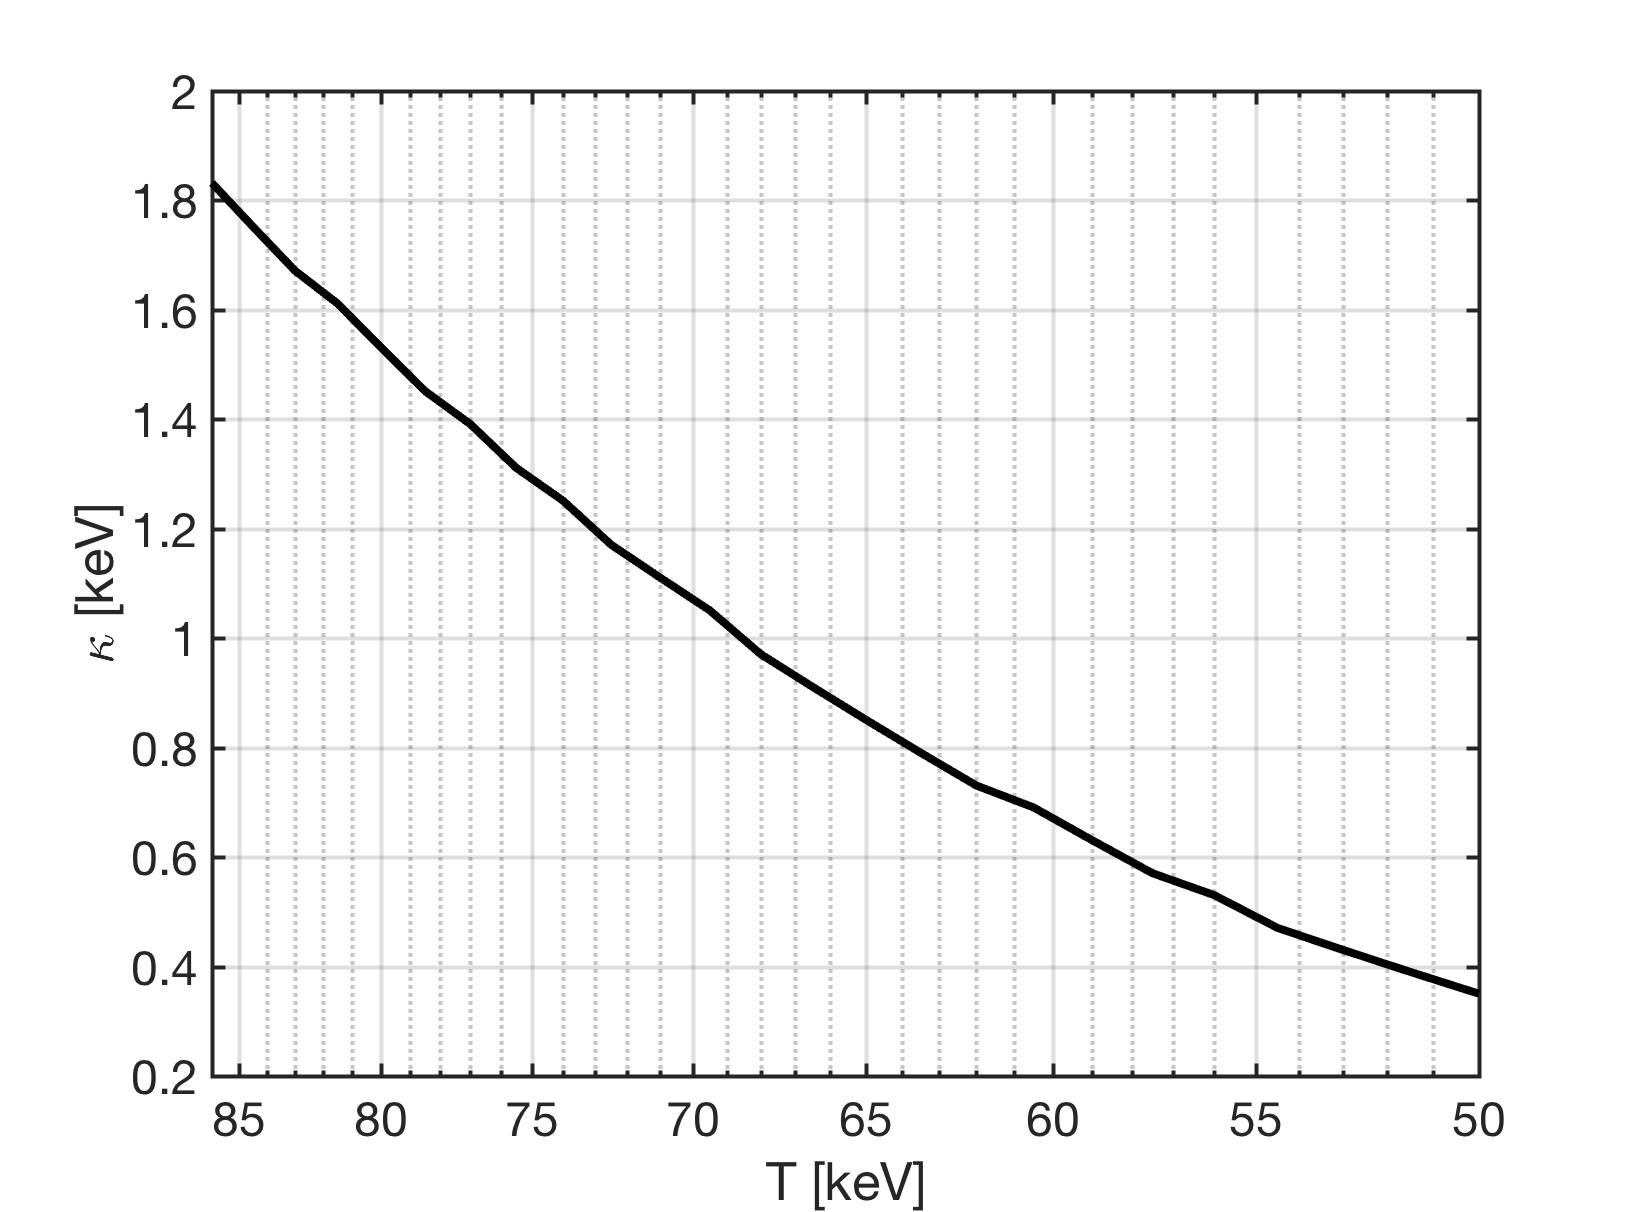
\includegraphics[width=0.9\textwidth]{./plots/OverdampingKappa.jpg}}
\caption{The relaxation rate $\kappa$ that satisfies \req{Numerical_eq} selfconsistently as a function of temperature $50\leqslant T\leqslant 86$\,keV. The minor fluctuations are due to limited numerical precision}
\label{KappaSol:fig} 
\end{figure}
%%%%%%%%%%%%%%%%%%%%%%%%%%%%%%%%%%%%%%%%%%

This first estimate of self-consistent plasma damping shows high sensitivity demonstrating the need for full self-consistent evaluation of damping  rate in plasma within context  of a well-defined, self-consistent approach, where both damping and photon properties in plasma are determined in a mutually consistent manner, a project which is well ahead of current state of the art and which is well beyond the scope of this report.  


%Chris' Screening ~~~~~~~~~~~~~~~~~~~~~~~~~~~~~~~~~~~~~~~~~~~~~~~~~~~~~~~~~~~~~~~~~~~~~~~~~~~~~~~~~~~~~~
%\subsection{Electron-positron plasma in BBN}\label{chap:bbn}


%%%%%%%%%%%%%%%%%%%%%%%%%%%%%%%%%%%%%%%%%%
\para{Electron positron plasma screening in BBN}\label{sec:Discussion}

In this chapter, we review \cite{Grayson:2023flr}, which applies the non-relativistic longitudinal polarization function to study the dynamics of the electron-positron plasma in the early Universe. In particular, we discussed the damping rate, the electron-positron to baryon density ratio, and their potential implications for Big Bang Nucleosynthesis (BBN) through screening within linear response theory. We derived an approximate analytic formula for the potential of a moving heavy charge in a collisional plasma in \req{eq:pos_point_DDS} describing screening effects previously found only numerically \cite{Hwang:2021kno}. Our analytic formula can be readily used to estimate the effect of screening on thermonuclear reactions using \req{eq:DDSenhance}. The correction to thermonuclear reactions due to damped-dynamic screening is small due to the low velocity of nuclei and a large amount of collisional scattering. This is in line with the findings of \cite{Hwang:2021kno}, who conclude that even though the densities are large, they are not enough to modify the potential at short distances related to screening. The analytic expression we find for the nuclear reaction rate enhancement \req{eq:DDSenhance} in a collisional plasma could be useful in other fusion environments such as stellar fusion and laboratory fusion experiments, such as those discussed in ~\cite{Labaune:2013dla,Margarone:2022mdpi}.

Overall we were very surprised to find that the screening effects in BBN were so small even in the static case, considering that the number densities present during BBN are $\sim 10^4$ times normal matter. If we compare this to screening effects on Earth, we can see that although plasmas occur at lower densities, they also occur in much colder environments. The strength of the screening effect is related to the Debye mass
\begin{equation}
m_D^2 \sim \frac{n_\text{eq} }{T}\,,
\end{equation}
which is on the order of a few keV during BBN. On earth, $n_\text{eq}$ is decreased by $\sim 10^4$, but T is decreased by $\sim 10^6$. Thus, we would expect to see similar, if not larger, screening effects on Earth. For instance, the Debye screening length in extracellular fluid in the body is 8 \AA ngstrom \cite{Wennerstrom:2020}, only a factor of $\sim 20$ times larger than the Debye length during BBN. We can have these large densities at low temperatures on earth due to gravity's agglomeration of matter in the universe.

%%%%%%%%%%%%%%%%%%%%%%%%%%%%%%%%%%%%%%%%%%%%%%%%
\para{The short-range screening potential}
In \cite{Grayson:2023flr}, a proposal is made to study the short-range potential relevant to quantum tunneling in thermonuclear reactions. Since the Gamow energy at which nuclei are most likely to tunnel is above the thermal energy, the portion of the screening potential relevant for tunneling does not satisfy the "weak-field" limit where the electromagnetic energy is small compared to the thermal energy
\begin{equation}
 \frac{q \phi(x)}{T} \ll 1\,.
\end{equation}
When this condition is not satisfied one must consider the full equilibrium distribution when calculating the short-range potential \cite{Hakim:1967prd,DeGroot:1980dk}
\begin{equation}\label{eq:Boltz}
 f_B^\pm(x,p) = e^{-(p_0\pm e\phi(x))/T}\,.
\end{equation}
The $e\phi$ term in the exponential accounts for the change in energy of a charge in the plasma due to its presence in an external field. For this equilibrium distribution, a linear response is no longer possible since the equilibrium distribution depends on the external electromagnetic field. In equilibrium one can find the static screening potential for strong electromagnetic fields using the nonlinear Poisson-Boltzmann equation,
\begin{equation}\label{eq:Poisson-Boltz}
 -\nabla^2 e\phi_{(\text{eq})}(x)/T +m_D^2\sinh\left[e\phi_{(\text{eq})}(x)/T\right] =e\rho_\mathrm{ext}(x)/T\,.
 \end{equation}
This equation has a well-known solution for an infinite sheet which we used to argue the importance of strong screening in BBN. 
In a future publication, we will solve the Poisson-Boltzmann equation with strong screening to calculate the short-range screening potential in BBN. We note that the toy model in \cite{Grayson:2023flr} overestimates strong screening effects for two reasons: an infinite sheet has a constant electric field requiring more polarizing charge density to screen the field, and the Boltzmann distribution in \req{eq:Boltz} does not account for the stacking of electron-positron states when the density of electrons and positrons becomes very large near the nucleus. Both of these effects significantly reduce the effect of strong screening on reaction rates, but at the time of writing, it seems that strong screening will create a larger effect on nuclear reaction rates than damped-dynamic screening. Predicting enhanced screening may be relevant for the anomalous screening observed in the measurements of astrophysical S(E) factors \cite{Zhang:2020nuc}.
 
%%%%%%%%%%%%%%%%%%%%%%%%%%%%%%%%%%%%%%%%%%%%%%%%%%%%%
\para{Early Universe plasma: non-relativistic polarization tensor}\label{sec:kinetic_theory}
The properties of the BBN plasma are described by the relativistic Vlasov-Boltzmann transport equations \req{eq:VBEf}. Since photons do not couple directly to the electromagnetic field, they do not contribute to the polarization tensor at first order in $\delta f$ as indicated in Eq.\,(\ref{eq:VBEg}). We neglect photon influence on the electron-positron distribution through the scattering term since the rate of inverse Compton scattering $R_{e^{\pm}\gamma }$ shown in green in \reff{RelaxationRate:fig} is much smaller, in the BBN temperature range, than the total rate $\kappa$ shown as a black line. Each fermion Boltzmann equation \req{eq:VBEf} can be solved independently. Since the equations for electrons and positrons are equivalent, except for the charge sign, only one needs to be solved to understand the dynamics.

%We do not consider the influence of light nuclei on the polarization tensor since their density during the BBN epoch is much smaller than that of electrons and positrons \reff{BBN_Electron}. One can see in \reff{MeanFreePath_fig} that the separation of baryons $n_B^{-1/3}$ in black is much larger than the size of the polarizing Debye sphere, so baryons do not participate significantly in screening.

We take the equilibrium one particle distribution function $\eq{f_\pm}$ of electrons and positrons to be the relativistic Fermi-distribution
\begin{equation}\label{eq:equildist}
\eq{f}_\pm(p) = \frac{1}{\exp{\left(\frac{\sqrt{\boldsymbol{p}^2 + m^2}}{T}\right)}
+1}\,,
\end{equation}
with chemical potential $\mu = 0 $. The electron and positron mass will be indicated by $m$ unless otherwise stated. At temperatures interesting for nucleosynthesis $T = 50-86$\,keV, we expect the plasma temperature to be much less than the mass of the plasma constituents. Only the non-relativistic form of Eq.\,(\ref{eq:equildist}) will be relevant at these temperature scales
\begin{equation}
\eq{f}_\pm(p) \approx \exp\left(- \frac{m}{T}\left(1+\frac{|\pmb{p}|^2}{2m^2}\right)\right)\,.
\end{equation}
Keeping terms up to quadratic order in $|\boldsymbol{p}|/m$ we solve the Vlasov-Boltzmann equation Eq.\,(\ref{eq:VBEf}) for the induced current and identify the polarization tensor. This is done in detail in our previous work in~\cite{Formanek:2021blc}.

% First, we expand Eq.\,(\ref{eq:VBEf})
% around small perturbations from equilibrium
% \begin{equation}\label{eq:perturbation0}
% f_\pm(x,p) = {\eq{f}_\pm}(p) + \delta f_\pm(x,p)\,,
% \end{equation}
% and solve \req{eq:VBEf} for $\delta f_\pm(x,p)$ in Fourier space. The induced current in Fourier space is given by
% \begin{equation}\label{eq:perturbation1}
% \tilde{j}_{\mathrm{ind}}^\mu(k) = 2\int \frac{d^4 p}{(2 \pi)^4}p^\mu 4\pi \delta_+(p^2-m^2) 
% \sum_{i = \, +, \, -} q_i \tilde{f}_{i}(k,p)\,,
% \end{equation}
% with the factor of two accounting for spin.
% After inserting \req{eq:perturbation0}, and specifying $q_\pm = \pm e$ the induced current is a function of the perturbation
% \begin{multline}\label{eq:perturbation2}
% \tilde{j}_{\mathrm{ind}}^\mu(k) = 2\int \frac{d^3 p}{(2 \pi)^3 p^0}p^\mu \Big( e \left[\eq{\tilde{f}}_+(k,p)-\eq{\tilde{f}}_-(k,p)\right]\\
% + e\left[\delta\tilde{f}_+(k,p)-\delta\tilde{f}_-(k,p)\right]
% \Big)
% \\
% =4 e\int \frac{d^3 p}{(2 \pi)^3 p^0}p^\mu \delta\tilde{f}(k,p)
% \,,
% \end{multline}
% because the equilibrium currents cancel in the weak field limit and the perturbations add since they differ by the charge $\delta f_\pm=\pm e \delta f' $. This term is studied for finite chemical potential in~\cite{Wang:2010px}. We focus on the second term related to the polarization response of the plasma.

% The polarization tensor can be obtained from \req{eq:perturbation2} by computing the 4-momentum integrals over $p$ in the rest frame of the plasma. Once integrated, the 4-potential $\widetilde{A}^{\nu}(k)$, coming from the electromagnetic field strength tensor $F^{\mu \nu}$ in \req{eq:VBEf}, factors out since it only depends on the 4-wavevector $k$ and \req{eq:perturbation2} attains the form of \req{eq:linresp}. For details, see Ref.~\cite{Formanek:2021blc}.

In the infinite homogeneous plasma filling the early Universe, the polarization tensor only has two independent components: the longitudinal polarization function $\Pi_{\parallel}$ parallel to field wave-vector $\boldsymbol{k}$ in the rest frame of the plasma and the transverse polarization function $\Pi_{\perp}$ perpendicular to $\boldsymbol{k}$~\cite{melrose2008quantum}. In the non-relativistic limit, these functions are~\cite{Formanek:2021blc}
\begin{align}\label{eq:polfuncs}
	\Pi_\parallel(\omega,\boldsymbol{k}) &= -\omega_p^2\frac{\omega^2}{(\omega+ i \kappa)^2} \frac{1}{1-\frac{i\kappa}{\omega+ i \kappa}\left(1+\frac{ T |\boldsymbol{k}|^2}{m (\omega+ i \kappa)^2} \right)}\,,\\
	\Pi_{\perp}(\omega) &= -\omega_p^2 \frac{\omega}{\omega+ i \kappa}\,.
\end{align}
In these expressions, the plasma frequency $\omega_p$ (defined as $m_L$ in~\cite{Formanek:2021blc}) is related to the Debye screening mass in the non-relativistic limit as
\begin{equation}\label{eq:plasmafreq}
 \omega_p^2 = m_D^2\frac{T}{m}\,.
\end{equation}

%%%%%%%%%%%%%%%%%%%%%%%%%%%%%%%%%
\begin{figure} 
\centerline{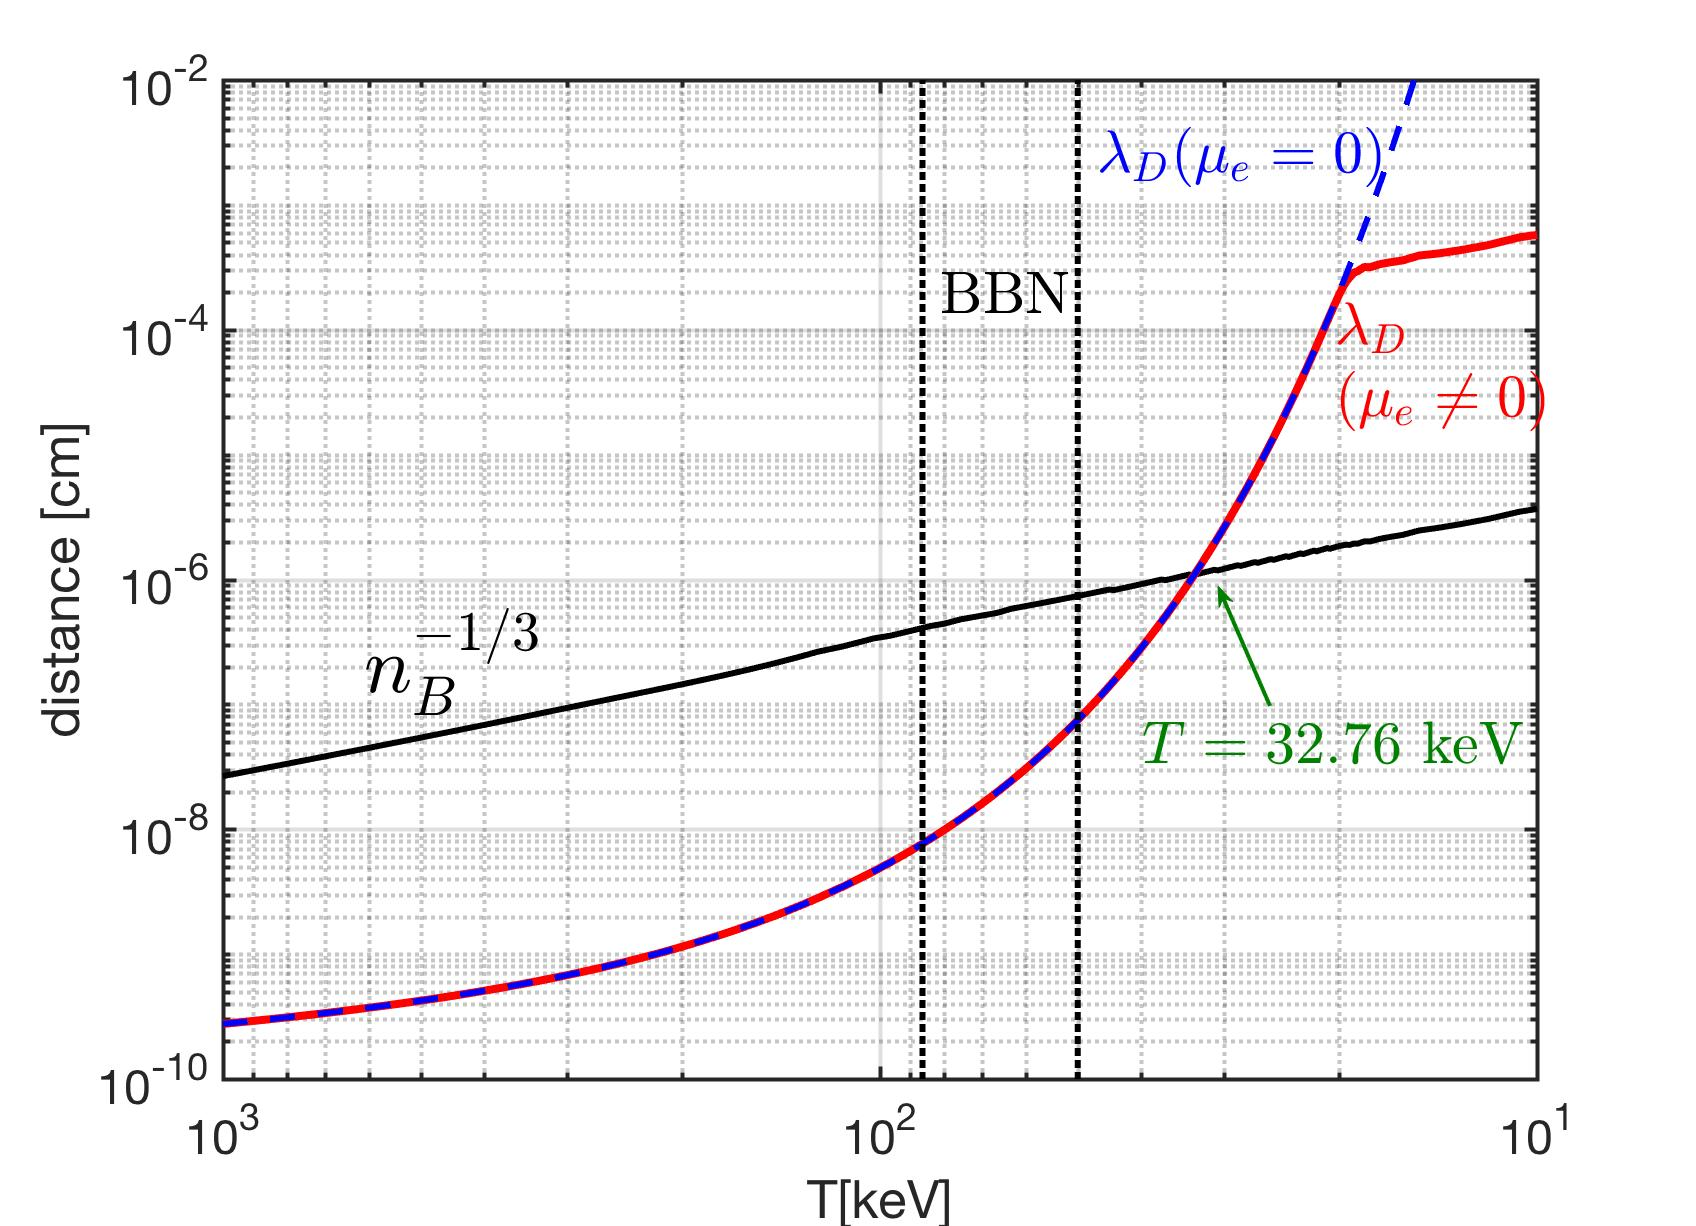
\includegraphics[width=0.90\linewidth]{plots/chap03BBN/Distance_Plasma002.jpg}}
\caption{ The average distance between baryons $n_B^{-1/3}$ and the Debye length $\lambda_D$ ($\mu_e \neq 0$) as a function of temperature (red solid line). During the BBN epoch (vertical dotted lines) $n_B^{-1/3}>\lambda_D$. For temperature below $T<32.76$ keV we have $n_B^{-1/3}<\lambda_D$. For comparison, the Debye length for zero chemical potential $\mu_e=0$ is also plotted as a blue dashed line. \cccite{Grayson:2023flr}}
\label{MeanFreePath_fig} 
\end{figure}
%%%%%%%%%%%%%%%%%%%%%%%%%%%%%%%%%%%%%%

The transverse response $\Pi_{\perp}$ relates to the dispersion of photons in the plasma. Here we need only consider $\Pi_\parallel$ since the vector potential $\boldsymbol{A}(t,\boldsymbol{x})$ of the traveling ion will be small in the non-relativistic limit. This work does not consider the effect of a primordial magnetic field discussed in~\cite{Steinmetz:2023abc}. We note that Debye mass $m_D$ is related to the usual Debye screening length of the field in the plasma as
\begin{equation}\label{eq:mL}
	1/\lambda_D^{2} = m_D^2= 4 \pi \alpha \left(\frac{2mT}{\pi}\right)^{3/2}\frac{e^{-m/T}}{2T}\,.
\end{equation}
This formula describes the characteristic length scale of screening in the plasma.

%%%%%%%%%%%%%%%%%%%%%%%%%%%%%%%%%%%%%%%%%%%%%
\para{Longitudinal dispersion relation}
As discussed in Chapter \ref{chap:PlasmaSF} the poles in the propagator or roots of the dispersion equation represent the plasma's propagating modes, often called `quasi-particles' or `plasmons.' In the non-relativistic limit, one can solve the longitudinal part of the dispersion equation \req{eq:disp}, which is relevant for finding charge oscillation modes in the plasma
\begin{equation}
    1+ \frac{\Pi_\parallel( k)}{(p\cdot u)^2}= 1+ \frac{\Pi_\parallel(\omega, \boldsymbol{k})}{\omega^2}=\varepsilon_\parallel(\omega,\boldsymbol{k}) =0 \,,
\end{equation}
evaluated in the rest frame. Then we insert \req{eq:polfuncs} to find
\begin{equation}
   1- \frac{\omega_p^2}{(\omega+ i \kappa)^2} \frac{1}{1-\frac{i\kappa}{\omega+ i \kappa}\left(1+\frac{T |\boldsymbol{k}|^2}{m(\omega+ i \kappa)^2} \right)}=0 \,.
\end{equation}
We can simplify the above expression since this is only a function of $\omega' =\omega+i\kappa$
\begin{equation}
   1- \frac{\omega_p^2}{\omega'^2-i\kappa\omega'+\frac{i\kappa T |\boldsymbol{k}|^2}{m \omega'} }=0 \,.
\end{equation}
Then we get a cubic equation for $\omega'(|\boldsymbol{k}|)$
\begin{equation}\label{eq:dispfact}
   \frac{1}{\omega'^3-i\kappa\omega'^2+\frac{i\kappa T |\boldsymbol{k}|^2}{m} }
    \left(\omega'^3-i\kappa\omega'^2 - \omega_p^2\omega'+\frac{i\kappa T |\boldsymbol{k}|^2}{m} \right)=0 \,.
\end{equation}
Cardano's formula gives the solutions to this cubic equation
\begin{equation}\label{eq:cardano}
\omega_n(\boldsymbol{k}) = \frac{1}{3}\left(i\kappa-\xi^n C-\frac{\Delta_0}{\xi^n C}\right), \qquad n \in \{0,1,2\} \,,
\end{equation}
with the quantities:
\begin{align}\label{eq:delta}
  \xi &=\frac{i\sqrt{3}-1}{2}\,,\\
    C &= \sqrt[3]{\frac{\Delta_1 \pm \sqrt{\Delta_1^2 - 4 \Delta_0^3}}2}\,,\\
    \Delta_0 &= -\kappa^2 + 3 \omega_p^2\,,\\
\Delta_1 &= 2i\kappa^3 - 9 i\kappa \omega_p^2 + 27\frac{i\kappa T |\boldsymbol{k}|^2}{m}.
\end{align}
Since the longitudinal dispersion relation is analytically solvable the full non-relativistic potential can be found in position space using contour integration. The residue of each pole will lead to the strength of that mode, and the location of the pole will lead to space and time dependence, which in simple cases is exponential. In practice, factoring out these roots in the Fourier transform of the potential leads to five poles, which do not seem to lead to simple expressions in position space. We found using the approximate expression derived in \req{sec:potential} was more practical. Deriving the full expression is the subject of future work.

%\begin{figure}[H]
%    \centering
%    \includegraphics[width=0.95\linewidth]{plasmafreq.png}
%    \caption{Plot of the plasma frequencies $\omega_\pm$ in the complex plane as a function of $\kappa$. At $\kappa=2\omega_p$ both solutions become imaginary, one becoming more quickly damped and the other more slowly damped.}
%    \label{fig:plasma-freq}
%\end{figure}

%%%%%%%%%%%%%%%%%%%%%%%%%%%%%%%%%%%%%%%%%%%%%%%%%%%%%%%%%
\para{Damped-dynamic screening} 
We discuss the application of the non-relativistic limit of the polarization tensor \rsec{chap:PlasmaSF} to the electron-positron plasma which existed during Big Bang nucleosynthesis (BBN)~\cite{Grayson:2023flr}. The BBN Epoch occurred within the first 20 min after the Big Bang when the Universe was hot and dense enough for nuclear reactions to produce light elements up to lithium \cite{Pitrou:2018cgg}. 

The BBN nuclear reactions typically take place within the temperature interval $86\, \mathrm{keV}>\mathrm{T_{BBN}}>50\, \mathrm{keV}$~\cite{Pitrou:2018cgg}. We refer to these elements produced in BBN as primordial light elements to distinguish them from those made later in the Universe's history. Primordial light element abundances are the most accessible probes of the early Universe before recombination. Though the current BBN model successfully predicts D, $^3$He, $^4$He abundances, well-documented discrepancies, such as $^7$Li, remain. Efforts to resolve the theoretical BBN model with present-day observations are discussed in detail in \cite{Pitrou:2021vqr,Bertulani:2022qly}.

A rather large electron-positron $e^-e^+$- number densities existed in the early Universe during Big Bang nucleosynthesis (BBN)~\cite{Wang:2010px,Hwang:2021kno,Rafelski:2023emw} are $10^2$ times larger than those present in the Sun \cite{Bahcall:2001smc} and $10^4$ times normal atomic densities \cite{Grayson:2023flr}. Charge screening is an essential collective plasma effect that modifies the inter-nuclear potential $\phi(r)$ changing thermonuclear reaction rates during BBN. An electron cloud around an ion's charge effectively diminishes the influence of nuclear charges beyond their immediate vicinity, lowering the Coulomb barrier. 

In the context of nuclear reactions, a reduced Coulomb barrier leads to a higher likelihood of penetration, boosting thermonuclear reaction rates. Consequently, this process influences the abundance of light elements in the early universe by modifying their formation rates. Since the BBN temperature range is much less than the electron mass, we will use the non-relativistic limit of the polarization tensor derived in Chapter \ref{chap:PlasmaSF}. The screened potential relevant for thermonuclear reactions will be given by the longitudinal polarization function \req{eq:phi}.

The influence of screening on nuclear reactions is a well-established field of study. The concept of plasma screening effects on nuclear reactions was initially introduced in~\cite{Salpeter:1954nc}, who suggested determining the increase in nuclear reaction rates through the use of the static Debye-Hückel potential~\cite{Debye:1923,Salpeter:1969apj,Famiano:2016hhs}. Subsequent research expanded this framework to account for the thermal velocity of nuclei traversing the plasma~\cite{Hwang:2021kno,Carraro:1988apj,Gruzinov:1997as,Opher:1999jh,Yao:2016cjs}, introducing the concept of `dynamic' screening. 

In our current study, we address the high density of the $e^-e^+\gamma$ plasma by including collisional damping using the current conserving collision term developed in \cite{Formanek:2021blc} shown in \req{eq:collision}. The dense aspect of the BBN plasma has only recently been acknowledged by incorporating collision effects into numerical models \cite{Sasankan:2019oee,Kedia:2020xdc}. We will refer to this model of screening as 'damped-dynamic' screening. In \cite{Grayson:2023flr}, we find an analytic formula for the induced screening potential, which allows for estimating the enhancement of thermonuclear reaction rates.

%%%%%%%%%%%%%%%%%%%%%%%%%%%%%%%%%%%%%%%%%%%%%%%%%%%%%%%%
\para{Nuclear potential}\label{sec:DDS}
We consider the effective nuclear potential for a light nucleus moving in the plasma at a constant velocity. This is done by Fourier transforming \req{eq:potentk}. The velocity of the nucleus is assumed to be the most probable velocity given by a Boltzmann distribution
\begin{equation}\label{eq:vel}
 \beta_{\text{N}} = \sqrt{\frac{2T}{m_N}}\,. 
\end{equation}
Since the poles of the \req{eq:potent} can be solved analytically, ideally, one would perform contour integration to get the position space field. Due to the intricacy of these poles $\omega_n(\boldsymbol{k})$, we find it insightful to look at the field in a series expansion around velocities of the light nuclei smaller than the thermal velocity of electrons and positrons and large damping.

% \begin{equation}
% \beta_{\text{N}}\frac{m_D}{\kappa} = \frac{v_{\text{N}}}{c}\frac{m_D}{\kappa} \ll 1\,.
% \end{equation}
\begin{equation}\label{eq:expansion}
% (\boldsymbol{k}\cdot\boldsymbol{\beta}_{\text{N}})^2 \ll \boldsymbol{k}^2 \frac{T}{m} \ll \kappa^2\, 
\frac{(\boldsymbol{k}\cdot\boldsymbol{\beta}_{\text{N}})^2}{\omega_p^2} \ll \frac{\boldsymbol{k}^2}{m_D^2} \ll \frac{\kappa^2}{\omega_p^2}\, .
\end{equation}


This expansion is useful during BBN since the temperature is much lower than the mass of light nuclei and the damping rate $\kappa$ is approximately twice the Debye mass $m_D$, as seen in Fig.~\ref{RelaxationRate:fig}. Applying this expansion to \req{eq:potentk} and evaluating this expression for a point charge $r \rightarrow 0$ we find
% % \begin{multline} \label{eq:potexp}
% % \phi(t,\boldsymbol{x}) = \phi_{\text{stat}}(t,\boldsymbol{x}) +\\ -Ze\int \frac{d^3\boldsymbol{k}}{(2\pi)^3} e^{ i\boldsymbol{k}\cdot(\boldsymbol{x}-\boldsymbol{\beta_{\text{N}}} t)}\frac{i \boldsymbol{k}\cdot \boldsymbol{\beta_{\text{N}}} m_D^2 (\frac{\boldsymbol{k}^2}{\kappa} - \frac{m}{T} \kappa)}{\boldsymbol{k}^2(\boldsymbol{k}^2+m_D^2)^2} e^{-\boldsymbol{k}^2\frac{R^2}{4}} \\ + O
% % \left(\beta_{\text{N}}\frac{m_D}{\kappa}^2\right)\,.
% % \end{multline}
% \begin{multline} \label{eq:potexp}
%  \phi(t,\boldsymbol{x}) = \phi_{\text{stat}}(t,\boldsymbol{x})\\ -Ze\int \frac{d^3\boldsymbol{k}}{(2\pi)^3} e^{ i\boldsymbol{k}\cdot(\boldsymbol{x}-\boldsymbol{\beta_{\text{N}}} t)}\frac{i \boldsymbol{k}\cdot \boldsymbol{\beta_{\text{N}}} m_D^4 (\frac{\boldsymbol{k}^2}{m_D^2} - \frac{\kappa^2}{\omega_p^2})}{\boldsymbol{k}^2(\boldsymbol{k}^2+m_D^2)^2\kappa} e^{-\boldsymbol{k}^2\frac{R^2}{4}} \,.
% \end{multline}
% First, we focus on the second term evaluating for a point charge $R\rightarrow 0$
\begin{equation}\label{eq:ddsint}
\phi(t,\boldsymbol{x}) =\phi_{\text{stat}}(t,\boldsymbol{x})-Ze\int \frac{d^3\boldsymbol{k}}{(2\pi)^3} e^{ i\boldsymbol{k}\cdot(\boldsymbol{x}-\boldsymbol{\beta_{\text{N}}} t)}\frac{i \boldsymbol{k}\cdot \boldsymbol{\beta_{\text{N}}} m_D^4 (\frac{\boldsymbol{k}^2}{m_D^2} - \frac{\kappa^2}{\omega_p^2})}{\boldsymbol{k}^2(\boldsymbol{k}^2+m_D^2)^2\kappa}\,.
\end{equation}
The second term is the damped-dynamic screening correction, which we refer to as $\Delta \phi$, where
\begin{equation}\label{eq:pos_point}
\phi(t,\boldsymbol{x}) = \phi_{\text{stat}}(t,\boldsymbol{x}) +\Delta \phi(t,\boldsymbol{x}) \,,
\end{equation}
and $\phi_{\text{stat}}$ is the standard static screening potential. The details of the integration of \req{eq:ddsint} can be found in \cite{Grayson:2023flr}, the result is
% In order to perform this integration we first note that this expression can be re-written as the laboratory time derivative
% \begin{equation}
%  \Delta\phi(t,\boldsymbol{x}) = Ze\frac{d}{dt}\left[\int \frac{d^3\boldsymbol{k}}{(2\pi)^3} e^{ i|\boldsymbol{k}||\boldsymbol{x}-\boldsymbol{\beta_{\text{N}}} t| \cos(\theta)}\frac{ m_D^4 (\frac{\boldsymbol{k}^2}{m_D^2} - \frac{\kappa^2}{\omega_p^2})}{\boldsymbol{k}^2(\boldsymbol{k}^2+m_D^2)^2\kappa}\right] \,,
% \end{equation}
% where the dot products were replaced by their angular dependence.
% The angular integration can be evaluated in spherical coordinates, see \ref{sec:static} for details,
% \begin{equation}
%  \Delta\phi(t,\boldsymbol{x}) = 2 Ze\frac{d}{dt}\left[\int \frac{d\boldsymbol{k}}{(2\pi)^2} \frac{\sin(|\boldsymbol{k}||\boldsymbol{x}-\boldsymbol{\beta}_N t|)}{|\boldsymbol{k}||\boldsymbol{x}-\boldsymbol{\beta}_N t|}\,\frac{ m_D^4 (\frac{\boldsymbol{k}^2}{m_D^2} - \frac{\kappa^2}{\omega_p^2})}{\boldsymbol{k}^2(\boldsymbol{k}^2+m_D^2)^2\kappa}\right] \,,
% \end{equation}
% \begin{multline}
%  \Delta\phi(t,\boldsymbol{x}) = \frac{Ze }{4\pi }\frac{m_D^2}{\kappa}\frac{d}{dt}\Bigg[\left(\frac{1+\nu_\tau^2}{ 2m_D}+\frac{\nu_\tau^2}{m_D^2 |\boldsymbol{x}-\boldsymbol{\beta}_N t|}\right)e^{-m_D |\boldsymbol{x}-\boldsymbol{\beta}_N t|}\\ - \frac{\nu_\tau^2}{m_D^2 |\boldsymbol{x}-\boldsymbol{\beta}_N t|} \Bigg]\,,
% \end{multline}
% here we introduce the ratio of the damping rate to the rate of oscillations in the plasma $\nu_\tau = \kappa/\omega_p$. We can apply the time derivative; note that
% \begin{equation}\label{eq:der_cos}
%  \frac{d}{dt} |\boldsymbol{x}-\boldsymbol{\beta}_N t| = - \frac{\boldsymbol{\beta}_N \cdot (\boldsymbol{x}-\boldsymbol{\beta}_N t)}{|\boldsymbol{x}-\boldsymbol{\beta}_N t|}= -\beta_N \cos(\psi)\,,
% \end{equation}
% where $\psi$ is the angle between $\boldsymbol{x}-\boldsymbol{\beta}_N t$ and $\boldsymbol{\beta}_N$. After taking the derivative and using the above expression \req{eq:der_cos} one finds

%%%%%%%%%%%%%%%%%%%%%%%%%%%%%%%%%%%%%
\begin{figure} 
 \centerline{
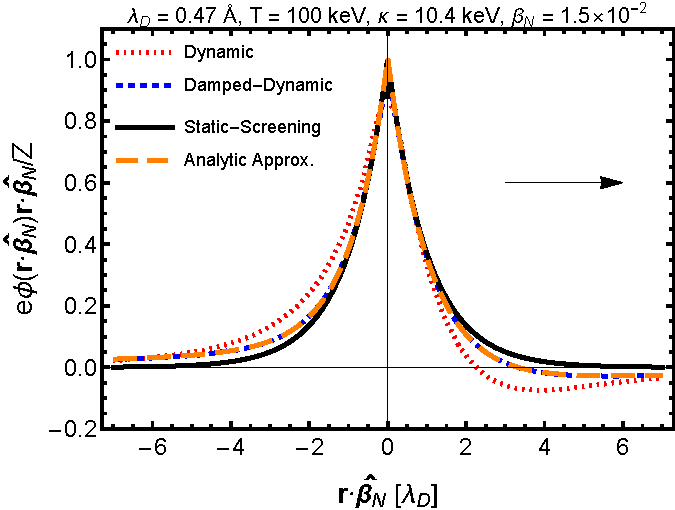
\includegraphics[width=.90\linewidth]{plots/chap03BBN/phidat_100_1_1_0_full_lin.pdf}}
 \caption{Plot of the total screening potential scaled with charge Z and distance along the direction of motion. We show a comparison of the following screening models plotted along the direction of motion of a nucleus $\boldsymbol{r}\cdot\hat{\boldsymbol{\beta}_{\text{N}}}$: static screening (black), dynamic screening (red dotted) from \cite{Hwang:2021kno}, damped-dynamic screening (blue dashed), and the approximate analytic solution of \req{eq:pos_point} (orange dashed). A black arrow indicates the direction of motion of the nucleus $\hat{\boldsymbol{\beta}_{\text{N}}}$. \cccite{Grayson:2023flr}}
 \label{fig:dynamiclinear}
\end{figure} 
%%%%%%%%%%%%%%%%%%%%%%%%%%%%%%%%%%%%%%%%%%%%

\begin{multline}\label{eq:pos_point_DDS}
\Delta \phi(t,\boldsymbol{x}) = \frac{Ze \beta_N \cos (\psi) m_D^2}{4 \pi \varepsilon_0 \kappa} \Bigg[\left(\frac{\nu_\tau^2}{m_D^2 r(t)^2} + \frac{\nu_\tau^2}{m_D r(t)}+\frac{1 + \nu_\tau^2}{2}\right)e^{-m_D r(t)} \\ -\frac{\nu_\tau^2}{m_D^2 r(t)^2}\Bigg]\,,
\end{multline}
where $\psi$ is the angle between $\boldsymbol{x}-\boldsymbol{\beta}_N t$ and $\boldsymbol{\beta}_N$ and $r(t) = |\boldsymbol{x}-\boldsymbol{\beta}_N t|$.
We introduce the ratio of the damping rate to the rate of oscillations in the plasma $\nu_\tau = \kappa/\omega_p$.  This expression is valid for large damping and slow motion of the nucleus or if the velocity of the nuclei is small. A similar result valid at large distances, which only includes the last term, was previously derived in~\cite{Stenflo:1973} for dusty (complex) plasmas. For large distances and large $\nu_\tau$, the last term in the second line is dominant, indicating that the overall potential would be over-damped. In this regime, the potential is heavily screened in the forward direction and unscreened in the backward direction relative to the motion of the nucleus. As $\nu_\tau$ becomes small, the $1/2$ in the first portion of the third term, proportional to $m_D^2/\kappa$, dominates. This flips the sign of the damped-dynamic screening contribution causing a wake potential to form behind the nuclei. This shift indicates the change from damped to undamped screening where \req{eq:pos_point_DDS} is no longer valid. 

%%%%%%%%%%%%%%%%%%%%%%%%%%%%%%%%%%
\begin{figure} 
 \centerline{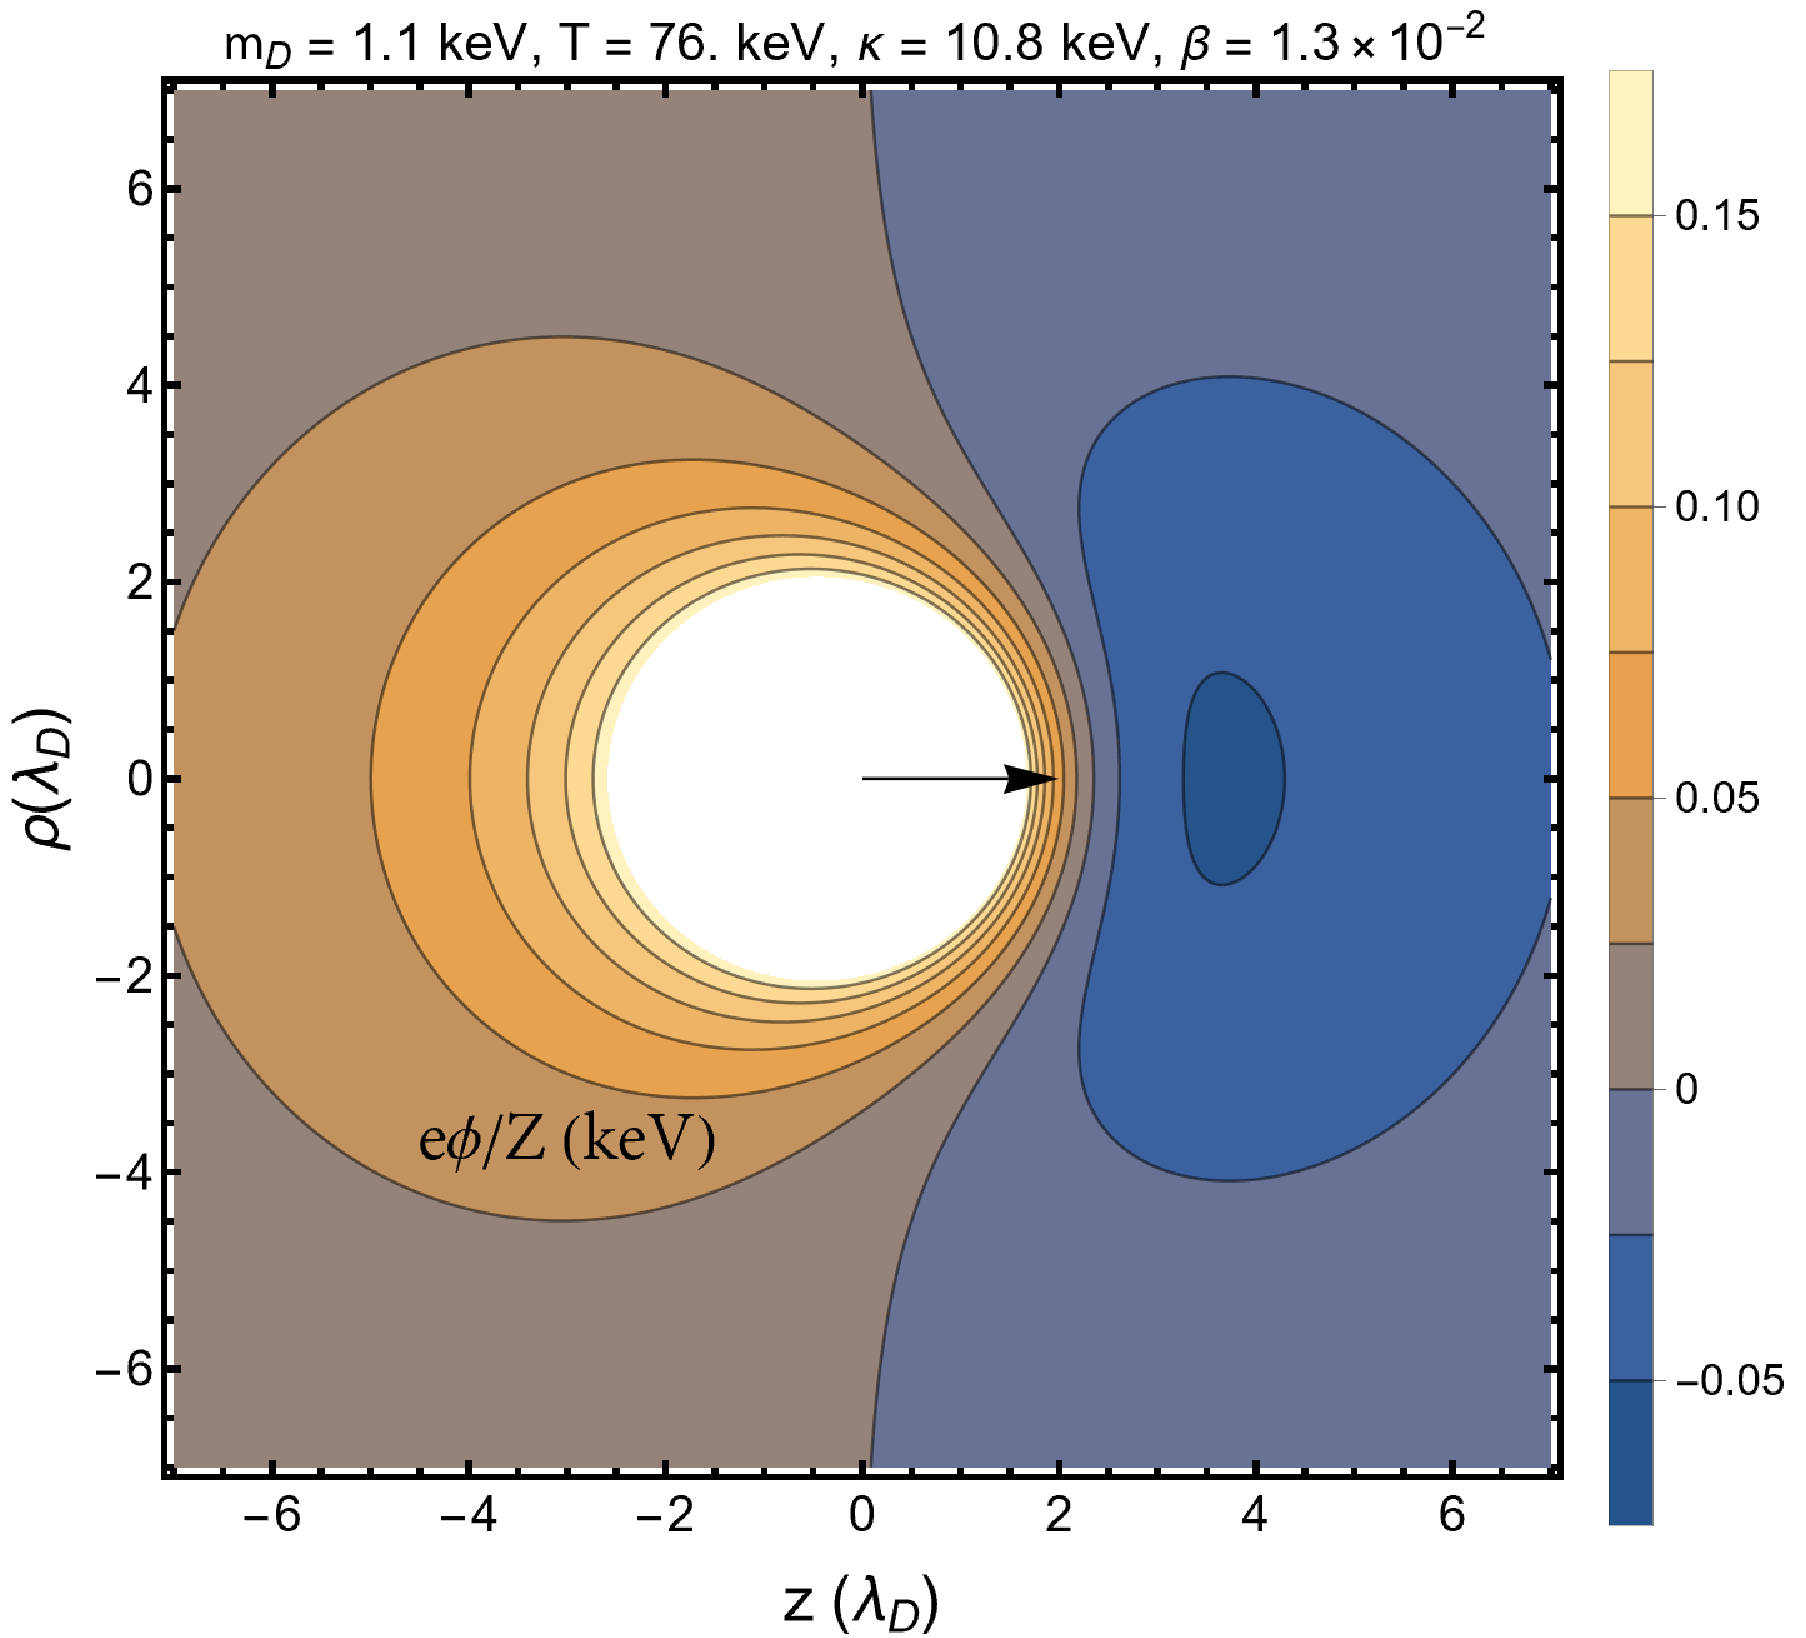
\includegraphics[width=.90\linewidth]{plots/chap03BBN/Pot_2DPlotFix.png}}
 \caption{Two dimensional plot of the total potential \req{eq:pos_point} scaled with Z, at $T=74\,$keV. The potential is cylindrically symmetric about the direction of motion $\boldsymbol{\hat{z}}$, which is indicated by a black arrow. The direction transverse to the motion is $\rho$. The sign of the damped-dynamic correction \req{eq:pos_point_DDS} changes sign due to the cosine term}
 \label{fig:numericalComp}
\end{figure} 
%%%%%%%%%%%%%%%%%%%%%%%%%%%%%%%%%%%%%

Figure~\ref{fig:dynamiclinear} demonstrates that the damped-dynamic response in the analytic approximation \req{eq:pos_point_DDS} (shown as orange dashed line) is sufficient to approximate the full numerical solution (blue dashed line) found by numerical integration of \req{eq:potent}. The temperature $T = 100$\, keV, above our upper limit of BBN temperatures, is chosen to relate to the dynamic screening result found in~\cite{Hwang:2021kno}. Our analytic solution differs from the numerical result in Fig.~4 of \cite{Hwang:2021kno} by a factor of $\sqrt{2}$ and is horizontally flipped. This reflection is due to a difference in convention in the permittivity, as seen in \req{eq:potentk}. We can see that dynamic screening is slightly stronger at large distances than damped screening, as expected. Damped and undamped screening are very similar at short distances, which is relevant to thermonuclear reaction rates. 

Dynamic screening in both the damped and undamped cases predicts less screening behind and more in front of the moving nucleus than static screening. This is shown in the two-dimensional plot \reff{fig:numericalComp}, of the total potential in plasma at $T=76\,$keV This effect was previously observed for subsonic screening in electron-ion-dust plasmas ~\cite{Stenflo:1973,Shukla:2002ppcf,Lampe:2000pop}. As a result, a negative polarization charge builds up in front of the nucleus. The small negative potential in front alters the potential energy between light nuclei, possibly changing the equilibrium distribution of light elements in the early universe plasma. This effect is much larger in the undamped case and is known in some cases to lead to the formation of dust crystals~\cite{Shukla:1996ccc}. 




%~~~~~~~~~~~~~~~~~~~~~~~~~~~~~~~~~~~~~~~~~~~~~~~~~~~~~~~~~~~~~~~~~~~~~~~~~~~~~~~~~~~~~~~




%%%%%%%%%%%%%%%%%%%%%%%%%%%%%%%%%%%%%
\subsection{Temperature Dependence of the Neutron Lifespan}
\para{Understanding Neutrons}\index{neutron}
Element production during BBN is influenced by several parameters, e.g. baryon to photon ratio $\eta_b$, number of neutrino species $N_\nu$, and neutron to proton ratio $X_n/X_p$, as controlled by both the dynamics of neutron freeze-out at temperature $T_f\approx 0.8\,\mathrm{MeV}$ and neutron lifetime.

Since about 200 seconds pass between neutron freeze-out, and midst of BBN neutron burn at $T\approx0.07\,\mathrm{MeV}$, the in plasma neutron lifetime is one of the important parameter controlling BBN element yields~\cite{Pitrou:2018cgg}. However, the neutron population dynamics and decay within the cosmic plasma medium with large abundances of neutrinos and $e^+e^-$-pairs is not the same as in effective vacuum laboratory environment. The medium influence on particle decay was discussed for example by Kuznetsova et al~\cite{Kuznetsova:2010pi}, we will further develop and use this method in order  to explore how cosmic primordial plasma influences neutron population dynamics.
 
After freeze-out when weak interaction scattering processes slow down to allow neutron abundance to free-stream,  neutron abundance remains  subject to natural decay
\begin{align}\label{Ndec}
n\longrightarrow p+e+\overline{\nu}_e\;.
\end{align}
The current experimental neutron lifetime remains method dependent, with a few second discrepancy, we adopt here the value  $\tau_n^0=880.2\pm1.0\,\mathrm{sec}$. However measurements  using magneto-gravitational traps unlike beam experiments offer a bit shorter value,  $877.7\pm0.7\,\mathrm{sec}$~\cite{Pattie:2017vsj}. In the standard Big-Bang nucleosynthesis (BBN) the neutron abundance when nucleosynthesis begins is assumed to be~\cite{Pitrou:2018cgg}
\begin{align}
\label{Xn_abundance}
X_n(T_{BBN})=X_n^f\exp\left(-\frac{t_{BBN}-t_f}{\tau_n^0}\right)\approx0.13\;,
\end{align}
The normalizing neutron freeze-out yield $X_n^f$ 
\begin{align}
\label{Xn_abundance2}
X_n^f \equiv  \frac{n_n^f}{n_n^f+n_p^f}= \frac{n_n^f/n_p^f}{1+n_n^f/n_p^f}\;.
\end{align}
where $n_n^f$ and $n_p^f$ are freeze-out neutron and proton densities, respectively. The thermal equilibrium yield ratio is
\begin{align}
\label{Xn_abundance3}
 \frac{n_n^f}{n_p^f}= \exp\left(-Q/T_f\right)\;,\qquad Q=m_n-m_p\;,
\end{align}
assuming a instantaneous freeze-out, depends on temperature $T_f$ at which neutrons decouple from the heat bath, and the neutron-proton mass difference (in medium). The values considered  are in the range $X_n^f=0.15\sim0.17$~\cite{Pitrou:2018cgg}. A dynamical approach to neutron freeze-out is necessary to fully understand $X_n^f$, we hope to return to this challenge in the near  future.

Following freeze-out the neutron is subject to natural decay and normally the neutron lifetime in vacuum $\tau_n^0$ is used c.f. Eq.\,(\ref{Xn_abundance}) to calculate the neutron abundance resulting in the \lq desired\rq\ value $X_n(T_{BBN})\approx0.13$ when BBN starts. To improve precision a dynamically evolving neutron yield needs to be studied and for this purpose we explore here the neutron decay which occurs in  medium, not vacuum. This leads to  neutron lifespan dependence on temperature of the cosmic medium as the decay occurs for a particle emerged in plasma of electron/positron, neutrino/antineutrino, (and protons).

Two physical effects of the medium  influence the neutron lifetime in the early universe noticeably:
\begin{itemize}
\item Fermi suppression factors from the medium: 
During the temperature range $T_f\geqslant T\geqslant T_{BBN}$, electrons and neutrinos in the background plasma can reduce the neutron decay rate by Fermi suppression to the neutron decay rate. Furthermore, the neutrino background can still provide the suppression after electron/positron pair annihilation becomes nearly complete.
\item Photon reheating:
When $T\ll m_e$ the electron/positron annihilation occurs, the entropy from $e^\pm$ is fed into photons, leading to photon reheating. The already decoupled (frozen-out) neutrinos remain undisturbed. Therefore, after annihilation we have two different temperatures in cosmic plasma: neutrino temperature $T_\nu$ and the photon and proton temperature $T$ respectively.
\end{itemize}
These two effect will be included in the following exploration of the neutron lifetime in the early universe as a function of $T$. We show how these effects alter the neutron lifespan and obtain the modification of the neutron yield at the time of BBN. Yet another effect was considered by Kuznetsova et al~\cite{Kuznetsova:2010pi} which is due to time dilation originating in particle thermal motion. In our case for neutrons with $T/m<10^{-3}$ this effect is negligible. Below we will explicitly assume that the neutron decay is studied in the neutron rest frame.

%%%%%%%%%%%%%%%%%%%%%%%%%%%%%%%%%%
\para{Decay Rate in Medium}
%\label{Rate_Medium}

The invariant matrix element for the neutron decay Eq.\,(\ref{Ndec}) for non-relativistic neutron and proton is given by
\begin{align}
\langle|\mathcal{M}|^2\rangle\approx16\,G^2_FV^2_{ud}\,m_nm_p(1+3g^2_A)(1+RC)E_{\bar{\nu}}E_e,
\end{align}
where the Fermi constant is $G_F=1.1663787\times10^{-5}\,\mathrm{GeV}^{-2}$, $V_{ud}=0.97420$ is an element of the Cabibbo-Kobayashi-Maskawa (CKM) matrix~\cite{Czarnecki:2018okw,Marciano:2005ec,Czarnecki:2004cw}, and $g_A=1.2755$ is the axial current constant for the nucleons~\cite{Czarnecki:2018okw,Marciano:2014ria}. We also consider the total effect of all radiative corrections relative to muon decay that have not been absorbed into Fermi constant $G_F$. The most precise calculation of this correction~\cite{Marciano:2014ria,Marciano:2005ec} gives $(1+RC)=1.03886$. 

In the early universe the neutron decay rate in medium, at finite temperature can be written as~\cite{Kuznetsova:2010pi}\index{neutron!decay rate in medium}
\begin{align}
\frac{1}{\tau^\prime_n}=\frac{1}{2m_n}\int&\frac{d^3p_{\bar{\nu}}}{(2\pi)^32E_{\bar{\nu}}}\frac{d^3p_p}{(2\pi)^32E_p}\frac{d^3p_e}{(2\pi)^32E_e}\notag\\
&(2\pi)^4\delta^4\left(p_n-p_p-p_e-p_{\bar{\nu}}\right)\langle|\mathcal{M}|^2\rangle\notag\\
&\big[1-f_p(p_p)\big]\big[1-f_e(p_e)\big]\big[1-f_{\bar{\nu}}(p_{\bar{\nu}})\big]\;,
\end{align}
where we consider this expression in the rest rest frame of neutron, {\it i.e.\/} $p_n=(m_n,0)$. The phase-space factors $(1-f_i)$ are Fermi suppression factors in the medium. The Fermi-Dirac distributions for electron and non-relativistic proton are given by
\begin{align}
&f_e=\frac{1}{e^{E_e/T}+1},\\
&f_p=e^{-E_p/T}=e^{-m_p/T}\,e^{-p_p^2/2m_pT}.
\end{align}
For neutrinos, after neutrino/antineutrino kinetic freeze-out they become free streaming particles. If we assume that kinetic freeze out occurs at some time $t_k$ and temperature $T_k$, then for $t>t_k$ the free streaming distribution function can be written as~\cite{Birrell:2012gg}
\begin{align}
f_{\bar{\nu}}=\frac{1}{\exp{\left(\sqrt{\frac{E^2-m_\nu^2}{T_\nu^2}+\frac{m^2_\nu}{T^2_k}}+\frac{\mu_{\bar{\nu}}}{T_k}\right)+1}},
\end{align}
for antineutrinos and we define the effective neutrino temperature $T_\nu$ as
\begin{align}
T_\nu\equiv\frac{a(t_k)}{a(t)}T_k.
\end{align}
In the following calculation, we assume the condition $T_k\gg\mu_{\bar{\nu}},\,m_\nu$, {\it i.e.\/} we consider the massless neutrino in plasma. Substituting the distributions into the decay rate formula and using the neutron rest frame, the decay rate can be written as 
\begin{align}
\label{Decay_rate_01}
\frac{1}{\tau_n^\prime}&=\frac{G^2_FQ^5V^2_{ud}}{2\pi^3}\,(1+3g^2_A)\,(1+RC)\\
&\times\int^1_{m_e/Q}d\xi\,\frac{\xi(1-\xi)^2}{\exp\left(-Q\xi/{T}\right)+1}\frac{\sqrt{\xi^2-(m_e/Q)^2}}{\exp\left(-Q(1-\xi)/T_\nu\right)+1},\notag
\end{align} 
where $Q$ was defined in Eq.\;(\ref{Xn_abundance3}) and we integrate using dimensionless variable $\xi=E_e/Q$. From Eq.(\ref{Decay_rate_01}), the decay rate in vacuum can be written as
\begin{align}
&\frac{1}{\tau_n^0}=\frac{G^2_Fm_e^5V^2_{ud}}{2\pi^3}(1+3g^2_A)\,(1+RC)\,f^\prime,
\end{align}
where the phase space factor $f^\prime$ is given by
\begin{align}
f^\prime&\equiv\left(\frac{Q}{m_e}\right)^5\int^1_{m_e/Q}d\xi\,{\xi(1-\xi)^2}\sqrt{\xi^2-(m_e/Q)^2}
\notag\\&=1.6360\,.
\end{align}

The phase space factor is also modified by the Coulomb correction between electron and proton, proton recoil, nucleon size correction etc. This has been studied by Wilkinson~\cite{Wilkinson:1982hu}, and the phase space factor is given by~\cite{Czarnecki:2018okw,Czarnecki:2004cw,Wilkinson:1982hu}
\begin{align}
f=1.6887.
\end{align}
These effect amount to adding the factor $\mathcal{F}$ to our calculation
\begin{align}
\mathcal{F}=\frac{f}{f^\prime}=1.0322,
\end{align}
then the neutron lifespan can be written as \index{neutron!lifespan in vacuum}
\begin{align}
\tau^{\mathrm{Vacuum}}_n=\frac{\tau^0_n}{\mathcal{F}}=879.481\,\mathrm{sec},
\end{align}
which compare well to the experiment result $877.7\pm0.7\,\mathrm{sec}$~\cite{Pattie:2017vsj}. 

In the case of plasma medium, we do not expect that these effect (Coulomb correction between electron and proton, proton recoil, nucleon size correction etc) are modified in the cosmic plasma. Thus we adapt the factor into our calculation and the neutron decay rate in the cosmic plasma is given by
\begin{align}
\label{Decay_rate_02}
&\frac{1}{\tau_n^{\mathrm{Medium}}}=\frac{G^2_FQ^5V^2_{ud}}{2\pi^3}\,(1+3g^2_A)\,(1+RC)\,\mathcal{F}\\
&\times\int^1_{m_e/Q}d\xi\,\frac{\xi(1-\xi)^2}{\exp\left(-Q\xi/{T}\right)+1}\frac{\sqrt{\xi^2-(m_e/Q)^2}}{\exp\left(-Q(1-\xi)/T_\nu\right)+1}.\notag
\end{align}
From Eq.(\ref{Decay_rate_02}) we see that the neuron decay rate in the early universe depends on both the photon temperature $T$ and the neutrino effective temperature $T_\nu$.

%%%%%%%%%%%%%%%%%%%%%%%%%%%%%%%%%%%%%%%%%%
\para{Photon Reheating}
%\label{Reheating}

After neutrino free-out and when $m_e\gg T$, the $e^{\pm}$ becomes non-relativistic and annihilate. In this case, their entropy is transferred to the other relativistic particles still present in the cosmic plasma, {\it i.e.\/} photons, resulting in an increase in photon temperature as compared to the freestreaming neutrinos. From entropy conservation we have
\begin{align}
\label{Entropy}
\frac{2\pi}{45}g^s_\ast(T_k)T^3_kV_k+S_{\nu}(T_k)=\frac{2\pi}{45}g^s_\ast(T)T^3V+S_{\nu}(T),
\end{align}
where we use the subscripts $k$ to denote quantities for neutrino freeze-out and $g^s_\ast$ counts the degree of freedom for relativistic species in early universe. After neutrino freeze-out, their entropy is conserved independently and the temperature can be written as
\begin{align}
T_\nu\equiv\frac{a(t_k)}{a(t)}T_k=\left(\frac{V_k}{V}\right)^{1/3}T_k.
\end{align}
In this case, from entropy conservation, Eq.(\ref{Entropy}), we obtain
\begin{align}
\label{Neutrino_Photon}
T_\nu=\frac{T}{\kappa},\,\,\,\,\,\,\kappa\equiv\left[\frac{g^s_\ast(T_k)}{g^s_\ast(T)}\right]^{1/3}.
\end{align}
From Eq.(\ref{Neutrino_Photon}) the neutron decay rate in a heat bath can be written as
\begin{align}
\label{Decay_rate_03}
&\frac{1}{\tau_n^\mathrm{Medium}}= \frac{G^2_FQ^5V^2_{ud}}{2\pi^3}(1+3g^2_A)\,(1+RC)\,\mathcal{F}\\
&\times\int^1_{m_e/Q}d\xi\,\frac{\xi(1-\xi)^2}{\exp\left(-Q\xi/{T}\right)+1}\frac{\sqrt{\xi^2-(m_e/Q)^2}}{\exp\left(-Q(1-\xi)\kappa/T\right)+1}.\notag
\end{align}

In the high temperature regime, $T\gg Q$, the exponential terms in the Fermi distribution becomes $1$ and the decay rate is given by
\begin{align}
&\frac{1}{\tau_n^\mathrm{Medium}}=\frac{1}{4}\left(\frac{1}{\tau_n^\mathrm{Vacuum}}\right)\;,
\qquad
T\gg Q\;.
\end{align}
In Fig.~\ref{Decay_Rate}, we plot the the neutron lifetime $\tau^\mathrm{Medium}_n$ in plasma as a function of temperature. Fermi-suppression from electron and neutrino increases the neutron lifetime as compared to value in vacuum. At low temperature, $T<m_e$, most of the electrons and positrons have annihilated and the main Fermi-blocking comes from the cosmic neutrino background. In this regime, the neutron lifetime depends also on the neutrino temperature, $T_\nu$. For cold neutrinos $T_\nu<T$, the Fermi suppression is smaller than the hot one $T_\nu=T$. 

%%%%%%%%%%%%%%%%%%%%%%%%%%%%%%%%%%%%%%%%%%%%%%%%%%%%%%%%%%%%%%%%%
\begin{figure} 
\centerline{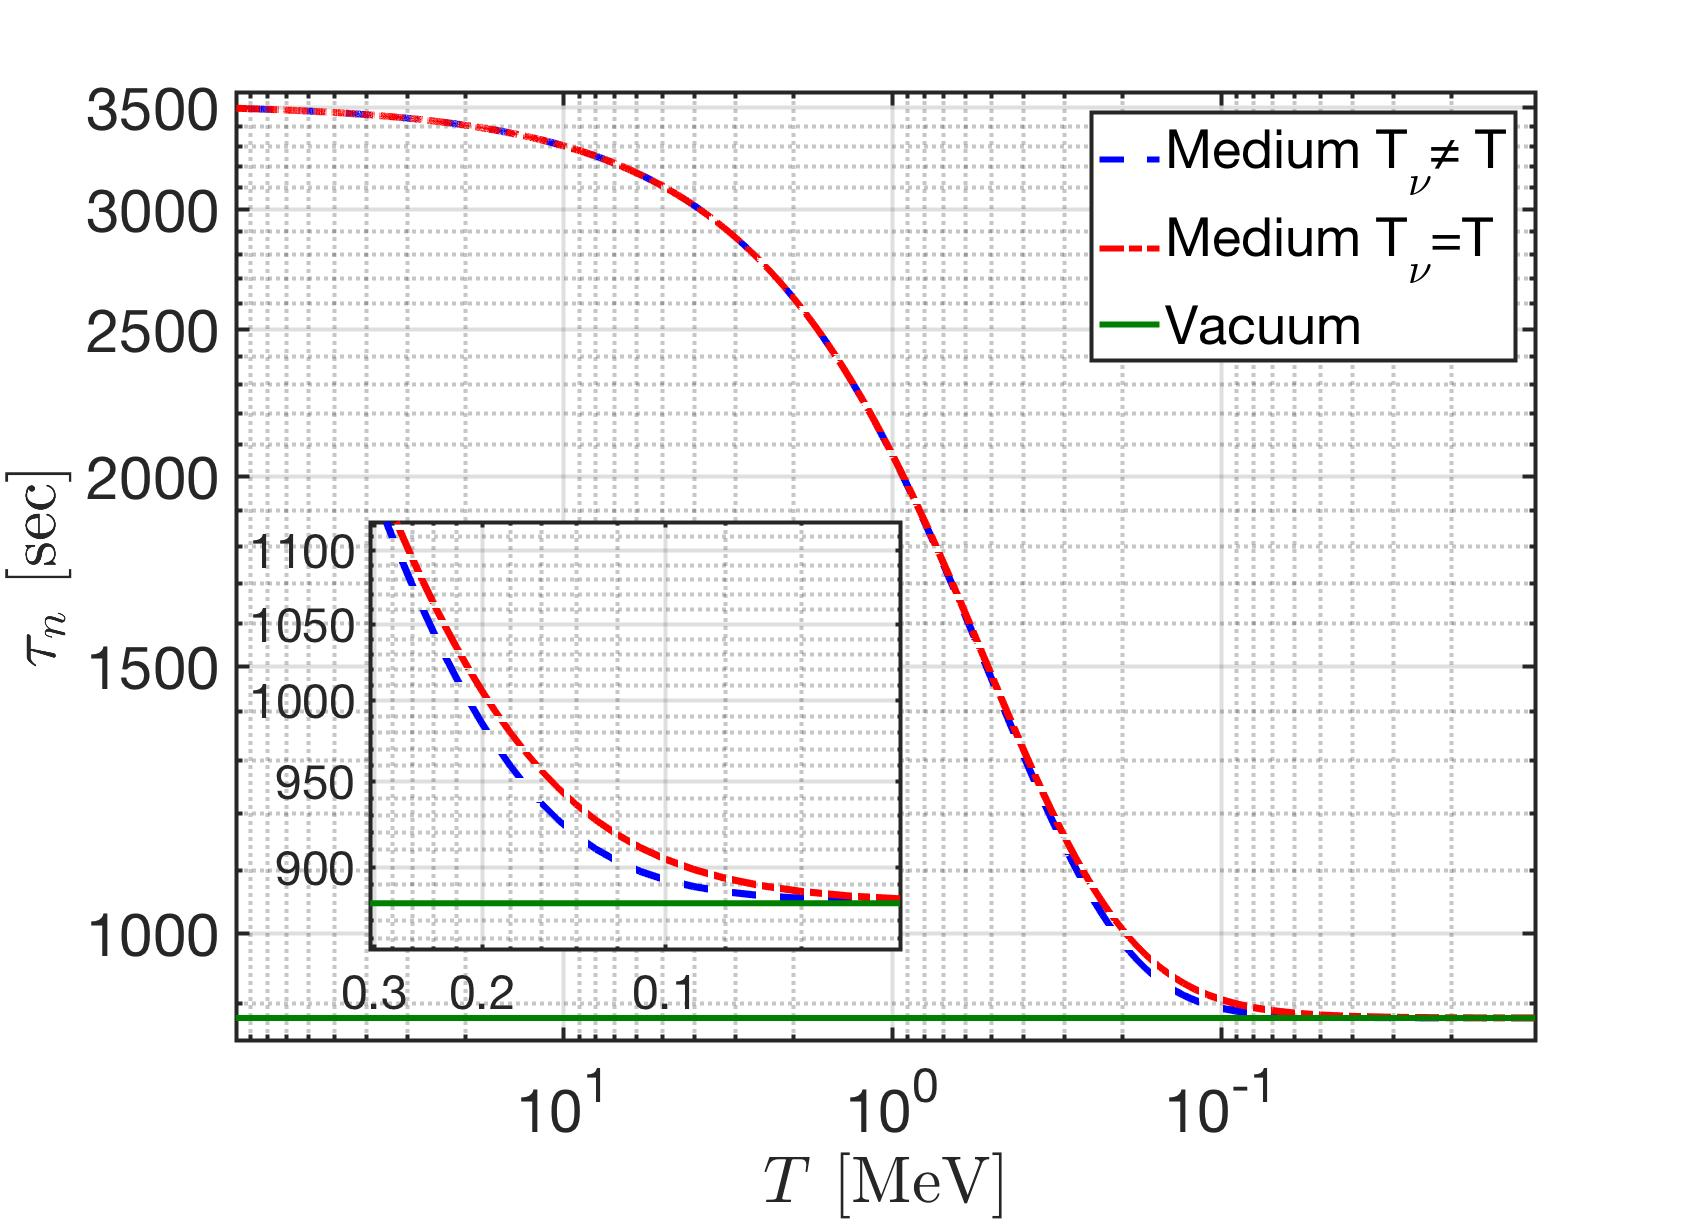
\includegraphics[width=0.9\textwidth]{./plots/Neutron_Lifetime_001}}
\caption{The neutron lifetime $\tau_n^\mathrm{Medium}$ in the cosmic plasma as a function of temperature. At high temperature $T=100\,\mathrm{MeV}$ the neutron lifetime is $3495\,\mathrm{sec}$ which is $3.974$ times larger than the lifetime in vacuum. At low temperature, $T<m_e$, the neutron lifetime depends also on the neutrino temperature, $T_\nu$, the effect is amplified in the insert} %Adapted from thesis of C.T.Yang~\cite{Yang:2024ret} }
\label{Decay_Rate} 
\end{figure}
%%%%%%%%%%%%%%%%%%%%%%%%%%%%%%%%%%%%%%%%%%%%%%%%%%%%%%%%%%%%%%%%%%

%%%%%%%%%%%%%%%%%%%%%%%%%%
\para{Neutron Abundance}
%\label{Neutron}

After the neutron freeze-out, the neutron abundance is only affected by the neutron decay. The neutron concentration can be written as \index{neutron! particle abundance}
\begin{align}
\label{Abundance}
X_n=X_n^f\,\exp\bigg[-\int^t_{t_f}\frac{dt^\prime}{\tau_n}\bigg],
\end{align}
where we use the subscripts $f$ to denote quantities at neutron freeze-out. Using Eq.(\ref{Decay_rate_03}) and Eq.(\ref{Abundance}), the neutron abundance ratio between plasma medium and vacuum is given by
\begin{align}
\label{Abundance_Ratio}
\frac{X_n^{\mathrm{Meduim}}}{X_n^{\mathrm{Vacuum}}}=\exp\bigg[-\int^t_{t_f}dt^\prime\left(\frac{1}{\tau^\prime_n}-\frac{1}{\tau^0_n}\right)\bigg].
\end{align}

In  \rf{Neutron:Abundance}, we plot the neutron abundance ratio as a function of temperature. Consider the neutron freeze-out temperature $T_f=0.08\mathrm{MeV}$ and the BBN temperature $T_{BBN}\approx0.07\mathrm{MeV}$, we found that the ratio ${X_n^{\mathrm{Meduim}}}/{X_n^{\mathrm{Vacuum}}}=1.064$ at temperature $T_{BBN}$. Then from Eq.(\ref{Xn_abundance}) the neutron abundance in plasma medium is given by
\begin{align}
X_n^{\mathrm{Meduim}}=1.064\,X_n^{\mathrm{Vacuum}}\approx0.138.
\end{align}
In this case, the neutron abundance will increase about $6.4\%$ in the cosmic plasma which should affect the final abundances of the Helium-4 and other light elements in BBN.
 
%%%%%%%%%%%%%%%%%%%%%%%%%%%%%%%%%%%%%%%%%%%%%%%%%%%%%%%%%%%%%%%%%%
\begin{figure} 
\centerline{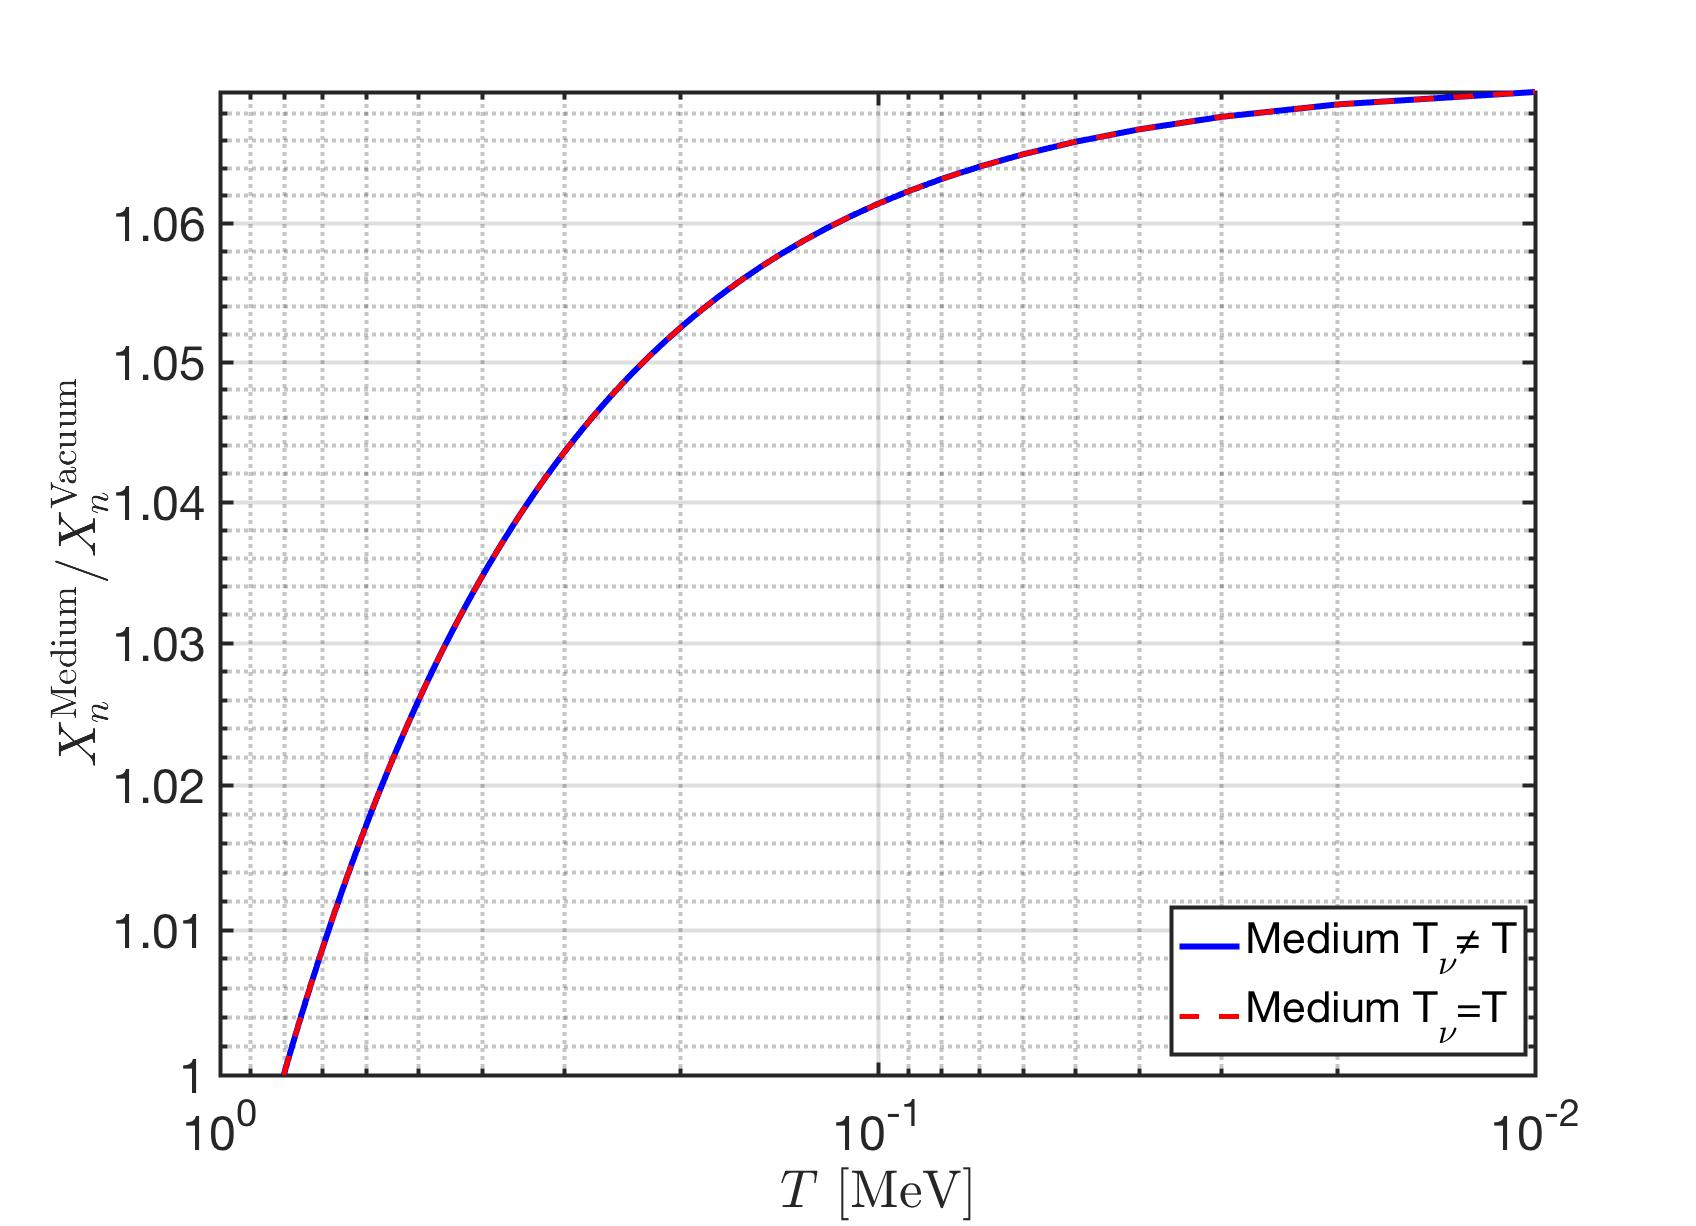
\includegraphics[width=0.9\linewidth]{./plots/Neutron_Abundance}}
\caption{The neutron abundance ratio as a function of temperature. Consider the neutron freeze-out temperature $T_f=0.08\mathrm{MeV}$ and the BBN temperature $T_{BBN}\approx0.07\mathrm{MeV}$, we find the abundance ratio ${X_n^{\mathrm{Meduim}}}/{X_n^{\mathrm{vacuum}}}=1.064$ at temperature $T_{BBN}$}% Adapted from thesis of C.T.Yang~\cite{Yang:2024ret} }
\label{Neutron:Abundance} 
\end{figure}
%%%%%%%%%%%%%%%%%%%%%%%%%%%%%

%%%%%%%%%%%%%%%%%%%%%%%%%%%%%%%%%%%%%%%%%%%%%%%%%%%%%%%%%%%%%%%%%%
%\section{Conclusion and Discussion}
%\label{Disscusion}
\para{How is BBN impacted?}
One of the important parameters of standard BBN is the neutron lifetime, as it affects the neutron abundance after neutron freeze-out at temperature $T_f\approx 0.8 \mathrm{MeV}$ and before the BBN $T\approx0.07 \mathrm{MeV}$. 

In the standard BBN model, it is necessary to have a neutron-to-proton ratio $n/p\approx1/7$ when BBN begins in order to explain the observed values of hydrogen and helium abundance~\cite{Pitrou:2018cgg}. We have evaluated the effect of Fermi suppression on the neutron lifetime due to the background electron and neutrino plasma. We found that in medium the neutron lifetime is lengthened by up to a factor 4 at a high temperature ($T>10$\,MeV). Our method should in principle also be considered in the study of medium modification of just about any of the BBN weak interaction rates, this remains a task for another day.

In the temperature range between neutron freeze-out just below $T=1$\;MeV and BBN conditions the effect of neutron lifespan is smaller but still noticeable. Near neutron freeze-out both decay electron and neutrino are blocked. However, after $e^\pm$ annihilation is nearly complete closer to BBN Fermi-blocking comes predominantly from the cosmic neutrino background and the neutron lifetime depends on the temperature $T_\nu<T$.

We found that the increased neutron lifetime results in an increased neutron abundance of ${X_n^{\mathrm{Meduim}}}/{X_n^{\mathrm{vacuum}}}=1.064$ at $T_{BBN}\approx0.07 \mathrm{MeV}$ {\it i.e.\/} we find a $6.4\%$ \emph{increase} in neutron abundance due to the medium effect at the time of BBN. We believe that this effect needs to be accounted for in the precision BBN study of the final abundances of hydrogen, helium and other light elements produced in BBN.
